
% options:
% thesis=B bachelor's thesis
% thesis=M master's thesis
% czech thesis in Czech language
% english thesis in English language
% hidelinks remove colour boxes around hyperlinks

\documentclass[thesis=M,english]{FITthesis}[2012/10/20]

% \usepackage[utf8]{inputenc} % LaTeX source encoded as UTF-8
% \usepackage[latin2]{inputenc} % LaTeX source encoded as ISO-8859-2
% \usepackage[cp1250]{inputenc} % LaTeX source encoded as Windows-1250

\usepackage{graphicx} %graphics files inclusion
%\usepackage{subfig}
\usepackage{amsmath}
\usepackage{amssymb}
\usepackage[chapter]{algorithm} % http://ctan.org/pkg/algorithms
\usepackage[noend]{algpseudocode} % http://ctan.org/pkg/algorithmicx
\usepackage{pseudocode}
\usepackage{comment}
\usepackage{enumitem}
\usepackage{amssymb}
\usepackage{caption}
\usepackage{subcaption}
\usepackage[section]{placeins}
\usepackage{dsfont}
\usepackage[utf8]{inputenc}

\usepackage[hang,flushmargin]{footmisc}
\usepackage{footnotebackref}


\usepackage{dirtree} %directory tree visualisation

% % list of acronyms
% \usepackage[acronym,nonumberlist,toc,numberedsection=autolabel]{glossaries}
% \iflanguage{czech}{\renewcommand*{\acronymname}{Seznam pou{\v z}it{\' y}ch zkratek}}{}
% \makeglossaries

%%%%%%%%%%%% own commands %%%%%%%%%%%%%%%%%%
\newcommand{\matr}[1]{\mathbf{#1}} 
\newcommand{\argmax}{\mathop{\mathrm{argmax}}}

\newcommand\footnoteref[1]{\protected@xdef\@thefnmark{\ref{#1}}\@footnotemark}

\makeatletter
\def\BState{\State\hskip-\ALG@thistlm}
\makeatother
%\newcommand{\max}{\mathop{\mathrm{max}}}

\raggedbottom

% % % % % % % % % % % % % % % % % % % % % % % % % % % % % % 
% EDIT THIS
% % % % % % % % % % % % % % % % % % % % % % % % % % % % % % 

\department{Department of Theoretical Computer Science }
\title{Learning Methods for Continuous-Time Hidden Markov Models}
\authorGN{Luk{\' a}{\v s}} %author's given name/names
\authorFN{Lopatovsk{\' y}} %author's surname
\author{Luk{\' a}{\v s} Lopatovsk{\' y}} %author's name without academic degrees
\authorWithDegrees{Bc. Luk{\' a}{\v s} Lopatovsk{\' y}} %author's name with academic degrees
\supervisor{Ing. Daniel Va{\v s}ata, Ph.D.}
\acknowledgements{I would like to express my gratitude to my supervisor Ing. Daniel Va{\v s}ata, Ph.D. for the useful comments, remarks and engagement through the learning process of this master thesis. Furthermore I would like to thanks to Ing. Tomáš Šabata for introducing me to this interesting topic and to the Datamole Ltd. for support of open-source development. }
\abstractEN{ The continuous-time hidden Markov model is promising not only for the biomedical research. The lack of efficient learning algorithms has limited its use in the past. However, recently the new efficient EM approaches were presented. In this thesis we are examining and comparing current state-of-the-art methods that are able to train models containing hundreds of hidden states. As the part of the work we have developed the general purpose continuous-time and discrete-time hidden Markov model library effectively implementing the best performing learning methods that is easy to use and available for everyone under open-source license. }

\abstractCS{ Skrytý Markovův proces se spojitým časem je slibným modelem s využitím nejen pro biomedicínský výzkum. Nedostatek efektivních algoritmů pro jeho učení v minulosti výrazne omezoval jeho použití. Nedávno však byly prezentovány nové efektivní metody založené na EM algoritmu. V této diplomové práci zkoumáme a srovnáváme současné moderní metody, které jsou schopné vycvičit modely obsahující až stovky skrytých stavů. Jako součást práce jsme vyvinuli univerzální knihovnu pro skrytý Markovův proces se spojitým a diskrétním časem, která efektivně implementuje nejslibnější učební metody. Knihovna je snadno použitelná a dostupná všem uživatelům pod licencí open-source.}
\placeForDeclarationOfAuthenticity{Prague}
\keywordsCS{ skrytý Markovův proces, skrytý Markovův proces se spojitým časem, strojové učení.}
\keywordsEN{ HMM, CT-HMM, hidden Markov model, continuous-time hidden Markov model, EM, HMMs, machine learning.}
\declarationOfAuthenticityOption{5} %select as appropriate, according to the desired license (integer 1-6)
\website{https://github.com/lopatovsky/DP} %optional thesis URL


\begin{document}

% \newacronym{CVUT}{{\v C}VUT}{{\v C}esk{\' e} vysok{\' e} u{\v c}en{\' i} technick{\' e} v Praze}
% \newacronym{FIT}{FIT}{Fakulta informa{\v c}n{\' i}ch technologi{\' i}}

\setsecnumdepth{part}

\begin{introduction}

A continuous-time hidden Markov model (CT-HMM) is a variant of hidden Markov model (HMM) where the output variables depend on the underlaying continuous-time Markov process. This differentiates it from the traditional HMM which is defined over discrete-time. 

The CT-HMM model can be used on datasets with irregular observation times where the state transitions are unobserved and usually occur in between of two observations. This makes the model stronger and applicable to much bigger set of problems comparing to discrete-time HMM which use is restricted to equidistant time sequences. The most of the research is currently performed over medical data. Patients undergo the examinations irregularly, while their inner health state could change multiple times in between of two visits of medical center. Use of the discrete-time model was insufficient. Quantification of time leads to the emission sequence where most of the observations are void. It also does not track possible changes of the states in between of two observations. The CT-HMM can effectively solve these issues. It was used successfully for prediction of disease interaction \cite{Le11}, modeling of glaucoma progression \cite{Li13, Li15}, and exploratory analyses of Alzheimer's Disease \cite{Li15}. Besides the medical field it was also used to predict the read and write operations arriving at a flash memory \cite{Zr10}.      

The cost for the higher flexibility of the model is more complex inference procedure. There are not just unknown hidden states in observation points but also unknown moments of state transition. The model parameter estimation showed to be a hard problem to solve. First attempts based on the direct maximizing of data likelihood and summing the probability through all possible hidden states have only worked for restricted number of hidden states or small number of allowed states transitions \cite{Zr10,Ja11}. There was a need for more effective learning algorithm with less limitations \cite{Li13}.    

The expectation maximization (EM) framework for the continuous-time Markov process and Bayesian networks in general was introduced in \cite{No12}. It was later extended to CT-HMM with the first proposed efficient EM algorithm in \cite{Li15}. The method is based on the computation of expected state transition and expected time spend in the state. It leads to the problem of solving integrals of matrix exponentials which is the most computationally demanding part of the method. Various approaches were used to solve it. Eigen decomposition (referred to as \textit{Eigen}) was used in \cite{Wa14} . However according \cite{Li15} it is not applicable for general jump-rate matrices which makes it unusable in practice. Two other methods were introduced in \cite{Li15}: direct truncation of the infinite sum expansion of the exponential (referred to as \textit{Unif}) and matrix exponentiation on an auxiliary matrix (referred to as \textit{Expm} ). The \textit{Unif} method was marked as unstable later in the article, whereas \textit{Expm} as being most robust and time efficient and able to compute models with hundreds of hidden states.      

There was an effective theoretical solution, but there was no publicly available implementation that would spread the technology towards general public. Our intention was to create first of its kind library implementing the state-of-the-art methods for CT-HMM, that would be moreover easy and fast to understand, and licensed as open source so it can be used and improved by everyone. 

As the result of this thesis, we have introduced the theory of the hidden Markov Models (Chapter  \ref{ch:pm}), described and explained the HMMs algorithms (Chapter \ref{ch:s}), implemented the general efficient HMM library for Python (details in Chapter \ref{ch:i}). The library effectively implements both discrete-time and continuous-time HMM. It provides all useful methods for work with the models as well as all algorithms described in the second chapter. Its key feature is the EM algorithm for continuous-time HMM parameters estimation. We have implemented more variants of \textit{Expm} algorithm. User can choose between \textit{soft} and \textit{hard} method \ref{sec:shm}, \textit{float-interval} and \textit{integer-interval} variant of algorithm \ref{sec:alg} and train with both full and sparse jump-rate matrix. The behavior of all implemented variants is examined by conducting  experiments (Chapter \ref{ch:e}).      
 	
\end{introduction}

\setsecnumdepth{all}

\chapter{Probabilistic Models}\label{ch:pm}

Before we start to talk about Continuous-time Hidden Markov Model (CT-HMM) we will briefly explain its discrete-time variant, usually just referred to as Hidden Markov Model (HMM or DT-HMM), starting by explaining the underlaying Markov process. This forms logical hierarchy as the CT-HMM is the natural extension of the discrete model sharing many ideas and subroutines, and Markov process is base building block of overall model. 

\section{Discrete-time Markov Process}\label{sec:DMP}
    
Discrete-time Markov process, also referred to as Markov chain, is the stochastic process $X_t$ in discrete equidistant time $\matr{T} = \{ 1, 2, 3 \dots \}$, that in every time-step occupies some state of the potentially infinite state set \cite{Gr01}. However, later in the text we restrict ourself on the finite state set $\mathcal{S} = \{ s_1, s_2, \dots, s_n\}$. The process being in time $t_i \in \matr{T}$ in the state $s_j$ will be denoted as $X_{t_i} = s_j$. Alternatively, to make some explanation simpler, we can also denote it just as $X_{t_i} = j$. The state of the process can change in every time-step. Probability that the process changed from state $s_i$ to state $s_j$ is called transition probability. We will refer to it as $a_{ij}$. The transition probabilities for all pairs of states form square matrix of size $n$ - the transition probabilities matrix $\matr{A}$ . Note that elements on its diagonal, although referred to as transition probabilities, represent the probabilities of the process remaining in the same state.

The Markov process is memory-less, not holding information about the past states. So the probability of next transition depends only on the current state. This characteristic is called the Markov property and can be expressed by the following equation.

\begin{equation}\label{eq:mp}
\begin{aligned}
\mathrm{P}(X_t & = s_j \mid X_{t-1} = s_i, X_{t-2} = s_k, \dots)  \\   
               & = \mathrm{P}(X_t = s_j \mid X_{t-1} = s_i ), \quad s_i,s_j,s_k \in \mathcal{S}, t \in \matr{T}
\end{aligned}
\end{equation}

If not stated differently, we will always refer to the time-homogeneous Markov processes. Homogeneity of the Markov process, described in following equation, guarantees that one step transition probabilities are not changing throughout the time so the matrix $\matr{A}$ stays constant. 

\begin{equation}\label{eq:homo}
   a_{ij} = \mathrm{P}(X_t = s_j \mid X_{t-1} = s_{j-1} ),\qquad 1 \leq i,j \leq n, \forall t
\end{equation}

 Standard stochastic constrains are applied for the transition probabilities \cite{Ra89}.

\begin{equation}
   a_{ij} \geq 0
\end{equation}

\begin{equation}
   \sum_{j=1}^n a_{ij} = 1
\end{equation}

\section{Discrete-Time Hidden Markov Model}\label{sec:dthmm}

The Discrete-time Hidden Markov Model (HMM) \cite{Ra89} is doubly embedded stochastic process consisting of underlaying discrete-time Markov process $X_t$ and another process $O$. The process $O$ assigns to every state $s_i$ the specific observation symbol from the set $\mathcal{V}$ that will be emitted by certain probability. The model is called ``hidden'', because the state sequence of Markov process is not directly visible. It can only be guessed from the measured observation symbols using statistical techniques. The set $\mathcal{V}=\{  v_1,v_2,\dots,v_m\}$ is a set of all observable (emission) symbols. The probability that state $s_i$ emits symbol $v_j$ or $\mathrm{P}( O_t = v_j  \mid X_t = s_i)$ will be denoted as $b_i(j)$ and together with other elements form the matrix $B$, rectangular matrix of $n$ rows and $m$ columns. Comparing to the single Markov process, HMM is able to model more complex systems, that can be closer to describe the processes of real life problems.  
  
The following parameters are needed to describe the HMM:

\begin{enumerate}[resume]
\setcounter{enumi}{0}
\item \textbf{Hidden States}
\begin{equation}
\mathcal{S} = \{ s_1,s_2, \dots, s_n \}
\end{equation} 
\item \textbf{State Transition Probability Matrix}
\begin{equation}\label{eq:tp}
\matr{A} = \{ a_{ij} \}, \quad 1 \leq i,j \leq n
\end{equation} 
\item \textbf{Observation Symbols}
\begin{equation}
\mathcal{V} = \{ v_1,v_2, \dots, v_m \} 
\end{equation}
\item \textbf{Observation Symbols Probability Matrix} \\
$\matr{B} = \{ b_{i}(k) \}$, where $b_{i}(k)$ is the probability that the observation $v_k$ will occur, if the system is currently in state $i$. 
\begin{equation}
b_i(k) = \mathrm{P}( O_t = v_k  \mid X_t = s_i), \qquad 1 \leq i \leq n, \quad 1 \leq k \leq m
\end{equation}
\item \textbf{Initial state distribution} \\
$\boldsymbol\pi = \{ \boldsymbol\pi_i \}$, where $\boldsymbol\pi_i$ is the probability of the initial state being $s_i$.
\begin{equation}
\boldsymbol\pi_{i} = \mathrm{P}(X_1 = s_i), \qquad 1 \leq i \leq n
\end{equation}
\end{enumerate}

For the convenience we will declare parameter $\boldsymbol{\theta} = (\matr{A},\matr{B},\boldsymbol\pi)$ compactly denoting the set of all parameters of the model. 

\section{Continuous-Time Markov Process}\label{sec:ctmp}

In the discrete-time Markov process described in Section \ref{sec:DMP} change of the current state of the process could only occur once we have moved a step further in the discrete time $t$. Comparing to this, in the continuous-time Markov process (CTMP) can change of state occur at any moment (the occurrence holds exponential distribution ).

%cit:[S.Karlin]
A finite state continuous-time Markov process is a~stochastic process $\{ X_t \mid t > 0\}$ on the states $\mathcal{S} = \{ s_1, s_2, \dots, s_n \}$  (for $n>0$ and $\mathcal{S}$ being the finite state set), that in any time $t$  occurs in corresponding state $x_t \in \mathcal{S}$. 

It satisfies the following properties for times $0 \leq u_0 < u_1 < \dots < u_r < u$ : 
\begin{description}
\item [Markov property:] Probability of transition from state $i$ to state $j$ during time interval $t$ is stationary i.e. independent on the states of process in the times $u^{'}$, $ u^{'} < u$.  
    
\begin{equation}
\begin{aligned}
& \mathrm{P}( X_{t+u} = s_j \mid X_u = s_i, X_{u_r} = s_{i_r}, \dots , X_{u_0} = s_{i_0} ) = \\ 
& = \mathrm{P}( X_{t+u} = s_j \mid X_u = s_i ), \qquad s_i,s_j,s_{i_0}, \dots ,s_{i_r} \in \mathcal{S} 
\end{aligned}
\end{equation}

The property describes that the stochastic process is memoryless.

\item [Homogeneity:] Probability of transition from state $s_i$ to $s_j$ in any given time $u \geq 0$ depends only on the length of the time interval $t \geq 0$. 

\begin{equation}
\begin{aligned}
& \mathrm{P}( X_{t+u} = s_j \mid X_u = s_i ) = \mathrm{P}( X_t = s_j \mid X_0 = s_i ) = \\
& = \mathrm{p_{ij}}(t)
\end{aligned}
\end{equation}

\end{description}
 

The upper mentioned conditions assert that the transition probability $\mathrm{p_{ij}}(t), i,j = 1,\dots,n$ satisfies following conditions \cite{Ka75}:


\begin{equation}
\mathrm{p_{ij}}(t) \geq 0,
\end{equation}

\begin{equation}
\sum_{j = 1}^n \mathrm{p_{ij}}(t) = 1,
\end{equation}

\begin{equation}\label{eq:ckeq}
\sum_{k = 1}^n\mathrm{p_{ik}}(u)\mathrm{p_{kj}}(t) = \mathrm{p_{ij}}(u+t).     
\end{equation}

Equation \eqref{eq:ckeq} is known as \textit{Chapman-Kolmogorov equation}. 
We can define the matrix $\matr{P_t}$, where the entry $(i,j)$ is $\mathrm{p_{ij}}(t)$ to get the equation in matrix form:

\begin{equation}\label{eq:ckm}
\matr{P_u} \matr{P_t} = \matr{P_{u+t}},   \qquad t,u > 0.  
\end{equation}

\subsection{ Jump Rates }

Using the \textit{Chapman-Kolmogorov equation} \eqref{eq:ckeq}, and if we know the probability $\mathrm{p_{ij}}(t)$ for every states $i,j$ and time $0 < t < t_0$, we are able to compute the values for any time $t > 0$ \cite{Ka75}. 

State transition probability $\mathrm{p_{ij}}(t)$ is continuous for $t=0$ \cite{Gr01}. After assigning $t=0$ we will get identity matrix $\matr{P_0} = \matr{I}$.
Moreover from \eqref{eq:ckm} follows that $\mathrm{p_{ij}}(t)$ is continuous for all $t>0$  and so that there exists the right derivative in 0. This knowledge enables us to determine the $\mathrm{p_{ij}}(t)$ for any given time $t>0$.   

\begin{equation}
q_{ij} =  \left.\frac{\mathrm{d}\mathrm{p_{ij}}(t)}{\mathrm{dt}} \,\right|_{t=0} 
\end{equation}

%= \lim_{t \to 0^+} \frac{\mathrm{p_{ij}}(t)}{t}, \quad \text{if } i\neq j     


We will call this derivative $q_{ij}$ the jump rate from state~$s_i$ to some other state~$s_j$. The jump rate $q_{ii}$ can be derived from the equation of transition probabilities summing to one.

\begin{equation}
1 = \mathrm{p_{ii}}(t) + \sum_{j = 1,j \neq i}^{ n } \mathrm{p_{ij}}(t) 
\end{equation}

Dividing it by time interval $t$ and letting $t$ decrease close to zero, we obtain the following equation. 

\begin{equation}\label{eq:qii}
 q_{ii} =  - \sum_{j = 1,j \neq i}^{ n} q_{ij} 
\end{equation}

We assume only finite rates $q_{ij}$. Infinite rate would immediately leave the state, so it makes no sense for us to consider.

It can be shown that by construction of the CTMP from discrete time Markov process (DTMP) \ref{sec:constr} and it's underlying Poisson process with rate $\lambda$ the equation $q_{ij} = \lambda a_{ij}$ holds. Where $a_{ij}$ is the transition probability from state $s_i$ to state $s_j$ in DTMP \ref{eq:tp}. This is why we call $q_{ij}$ the jump rate \cite{Gr01}.  

We can also look at $q_{ii}$ as at the rate in which the $X_t$ is leaving state $s_i$ \eqref{eq:ckeq}. We define the jump-rates matrix as $\matr{Q}(i,j) = q_{ij}$.

To get transition probabilities for any time $t$ from matrix $\matr{Q}$ we need to solve the \textit{Kolmogorov's Backward} equation 

\begin{equation}\label{eq:kbe}
\matr{P_t^{'}} = \matr{Q} \matr{P_{t}},
\end{equation}

\textit{Kolmogorov's Forward} equation. They can be obtained from \textit{Chapman-Kolmogorov equation} \eqref{eq:ckm} by differentiation \cite{Gr01}. The solution of the differential equation with the initial condition $\matr{P_0} = \matr{I}$ leads to following matrix exponentiation formula. 


\begin{equation}\label{eq:mexp}
\matr{P_{t}} = e^{\matr{Q}t}  
\end{equation}

%Such a defined matrix will hold $\pi\matr{Q} = 0$... [explain more, proof, $e^{\matr{Q}t}$]

\subsection{Construction from Discrete-Time Markov Process with Poisson Process Timing }\label{sec:constr} 

The useful way for understanding the continuous-time Markov process is to know its relation to the discrete process that can be shown by the following construction \cite{Gr01}.

We will take a homogeneous Poisson process $N(t)$ with parameter $\lambda$ and a discrete-time Markov process $Y_{\nu}$ with states transition probabilities $a_{ij}$. We assume the $N(t)$ and $Y_{\nu}$ being mutually independent. By changing equidistant timing of $Y_{\nu}$ to Poisson process timing, we will get the process $Y_{N(t)}$ in which transition from state $s_i$ happens at each arrival in $N(t)$ with probability $a_i = \sum_{j = 1}^{ n ,j \neq i} a_{ij}$. Notice that the transition will not occur if $i=j$. Similarly, the time spent in state $s_i$ before the transition occurs can be described by probability density function of exponential distribution with the parameter $\lambda a_i$ as $\mathrm{f}(t)= \lambda a_i e^{- \lambda a_i t}$. Such a process $X_t = Y_{N(t)}$ fulfills the CTMP definition as described in Section \ref{sec:ctmp}. 

Now we can derive the equation for probability of transition from state $s_i$ to state $s_j$ in the time $t$ as the sum of all possible numbers of steps in which the transition can occur. 

\begin{equation}
\begin{aligned}
\mathrm{p_t(i,j)} &= \sum_{n=0}^{\infty} \mathrm{P}( N(t) = n, X_t = s_j \mid X_0 = s_i )  = \\
                  &= \sum_{n=0}^{\infty} \mathrm{P}( N(t) = n, Y_{N(t)} = s_j \mid Y_{N(0)} = s_i )  = \\
                  &= \sum_{n=0}^{\infty} \mathrm{P}( N(t) = n ) \mathrm{P}( Y_n = j \mid Y_0 = i )  = \\
				  &= \sum_{n=0}^{\infty} e^{-\lambda t} \frac{ (\lambda t)^n}{n!} a_{ij}^n  
\end{aligned}
\end{equation} 

By differentiation of $ \mathrm{p_t(i,j)} $ with respect to $t$ at $0$, we get the following equation for jump-rate matrix $\matr{Q}$.  

\begin{equation}
\matr{Q} = \lambda( \matr{A} - \matr{I} )
\end{equation}



\subsection{ Fully Observable Continuous-Time Markov Process }


Let's have continuous time Markov process on the state space $\mathcal{S}$ with the jump rates in the matrix $\matr{Q}$, initial state probability distribution $\boldsymbol\pi$, and the known hidden state sequence $\matr{X^{'}}= ( x_0^{'}, x_1^{'}, \dots, x_{\nu^{'}}^{'} ) $ occurring with transitions in times $\matr{T^{'}} = ( t_0^{'}, t_1^{'}, \dots, t_{\nu^{'}}^{'} )$. Such a system in which we know when and where the transition will happen is called fully observable \cite{Li15}. We can count its complete likelihood $\mathcal{L}_{FO}$ what is the probability of state sequence $\matr{X^{'}}$ and time sequence $\matr{T^{'}}$ being generated by model with parameters $\matr{Q}$. 

\begin{equation}\label{eq:CL1}
\begin{aligned}
 \mathcal{L}_{FO} &= \mathrm{P}(X_{t_0^{'}}^{'} = x_0^{'}, \dots ,X_{t_{\nu}^{'}}^{'} = x_\nu^{'} \mid \matr{Q} ) = \\ 
 &=  \prod_{u=0}^{\nu^{'}-1} ( q_{x_u^{'} x_{u+1}^{'}} / q_{x_u^{'}} )( q_{x_u^{'}} e^{ - q_{x_u^{'}} \tau_{u }^{'}}) = \\
    &= \prod_{u=0}^{\nu^{'}-1} q_{x_u^{'} x_{u+1}^{'}} e^{ - q_{x_u^{'}} \tau_{u}^{'}}
\end{aligned}
\end{equation}

where $q_i = \sum_{j=1}^{n,i\neq j} q_{ij}$ is the probability of transition from state~$i$ and   
$\tau_{u}^{'} = t_{u+1}^{'} - t_{u}^{'}$ is the time interval among two consecutive steps.

The equation can be further rearranged into form that group together same state transition.  Variable $\eta_{ij}$ marks the number of transition $q_{ij}$ that have occurred and $\tau_i$ is the total time spend in state~$s_i$.

\begin{equation}\label{eq:CL2}
 \mathcal{L}_{FO} = \prod_{i=1}^{n} \prod_{j=1,i \neq j}^{n} q_{ij}^{\eta_{ij} } e^{ - q_i \tau_i }
\end{equation}

\subsection{ General Continuous-Time Markov Process }

In general we do not know states of the system during all the time. It is only known at some unevenly distributed times of observations $\matr{T} = ( t_0, t_1, \dots, t_{\nu} )$ as $\matr{X}= (x_0, x_1, \dots, x_{\nu} )$. 
This add an amount of insecurity in the probability computation. We do not longer know, the number of transitions $\eta_{ij}$ as well as the time spend in the specific state $\tau_i$. 

To count the likelihood of the process \cite{Li15}, we use earlier defined matrix $\matr{P}(t)$ and its elements $\mathrm{p_{ij}}(t)$ \ref{sec:ctmp}. The time interval among two observation is marked as  $\tau_u = t_{u+1} - t_u$.    

\begin{equation}
 \mathcal{L} = \mathrm{P}(X_{t_0} = x_0, \dots ,X_{t_\nu} = x_\nu \mid \matr{Q} ) = \prod_{u=0}^{\nu-1} \mathrm{p}_{x_u x_{u+1}}(\tau_u) 
\end{equation}

It can be alternatively extended in the form

\begin{equation}
 \mathcal{L} = \prod_{u=0}^{\nu-1} \prod_{i=0,j=0}^{n}  \mathrm{p}_{ij}(\tau_u)^{\mathds{1}( x_u = s_i, x_{u+1} = s_j )} 
\end{equation}

where function $\mathds{1}(i,j)$ equals either $1$, if both condition inside are true, or $0$ if they are not. 
We define $r$ as the number of all distinct time intervals from the set $ \matr{T}_{\Delta} = \{ \tau_1,\tau_2,\dots,\tau_r\}$. In case of $r$ being lower then the number of observations it can be beneficial to aggregate them as in formula

\begin{equation}\label{eq:CTL}
 \mathcal{L} = \prod_{\Delta = 1}^{r} \prod_{i=0,j=0}^{n}  \mathrm{p}_{ij}(\tau_{\Delta})^{\mathbb{C}( \tau=\tau_{\Delta}, x_u = s_i, x_{u+1} = s_j )} 
\end{equation}

where function $\mathbb{C}$ denotes to total number of intervals for which is the condition true.
    
\section{Continuous-Time Hidden Markov Model}\label{sec:cthmm1}

Continuous-time hidden Markov model is an extension of CTMP \ref{sec:ctmp} where states in times $\matr{T} = ( t_0, t_1, \dots, t_{\nu} )$ are not directly observed but just seen as the observation symbols sequence $\matr{O} = (  o_0, o_1, \dots, o_{\nu} )$ emitted by the current state $s_i$ with the probability $b_i(o)$. 

Emissions of the observable symbol can occur at any time independently on the state transition times. For example it could be times when patient undergoes medical examination. The times can generally have highly irregular and unbalanced distribution.

The likelihood of completely observed system $\mathcal{L}_{FO}$ is similar to the $\mathcal{L}_{FO}$ of CTMP \eqref{eq:CL1} \eqref{eq:CL2} with the difference we need to take into account the probability of actual observation.

\begin{equation}\label{eq:HMCL1}
\begin{aligned} 
			\mathcal{L}_{FO} &= \mathrm{P}(X_{t_0} = x_0, \dots ,X_{t_\nu} = x_\nu, O_{t_0} = o_0, \dots ,O_{t_\nu} = o_\nu \mid \matr{Q}, \matr{B} ) = \\
  &= \prod_{u^{'}}^{\nu^{'}-1} q_{x_{u^{'}} x_{u^{'}+1}} e^{ - q_{x_{u^{'}}} \tau_{u^{'}} } 
    \prod_{u=0}^v b_{ x_u }(o_u) = \\
    &= \prod_{i=1}^{n} \prod_{j=1, i \neq j}^{n} q_{ij}^{\eta_{ij} } e^{ - q_i \tau_i } \prod_{u=0}^\nu b_{x_u}(o_u)
\end{aligned}
\end{equation}

There is much more latent information in such defined model. Not just the hidden states, but also the unknown transition times and unknown state sojourn time (how long will the system remain in the state).
Sometimes state can change, without emitting a single observation. The large number of hidden information make it to be more complex problem then the discrete time model.

\chapter{Statistics}\label{ch:s}


\section{Expectation-Maximization Algorithm}\label{ch:EM}

Expectation-maximization (EM) algorithm (first introduced in \cite{De77}) is the method for finding the maximum likelihood estimates(MLE) of parameters in probabilistic models over incomplete data-set, i.e. data-set containing unobserved (latent) variables. It is a natural generalization of maximum likelihood estimation. However, the latent variables make finding of the MLE more difficult. Direct count can be very computationally expensive. The EM algorithm uses iterative approach to approximate the solution by repeating sequence of simpler consecutive steps.

Let's have $\mathbf{x} = (x_{1},x_{2},\dotsc,x_{n})$ containing the known (observed) variables and the vector $\mathbf{z} = (z_{1},z_{2},\dotsc,z_{n})$ containing latent (unobserved) variables. We set $\boldsymbol{\theta}$ for unknown parameters we want to estimate. We denote notation $\mathcal{L}(\mathbf{x},\mathbf{z}; \boldsymbol{\theta}) = \mathrm{P}(\mathbf{x},\mathbf{z} | \boldsymbol{\theta})$ for likelihood function which estimates the probabilities for given parameters. We can count MLE directly by summing through all possible values of latent variables $\matr{z}$ as in following equation $\mathcal{L}(\mathbf{x};\boldsymbol{\theta}) = \mathrm{P}(\mathbf{x} | \boldsymbol{\theta}) = \sum\limits_{\matr{z}} \mathrm{P}(\mathbf{x},\mathbf{z} | \boldsymbol{\theta})$ or get its approximation by EM algorithm in following steps \cite{Li14}.
%Notice that we are using the log-likelihood to avoid underflow of parameters values that could otherwise easily arise during the computation.  

\begin{enumerate}
\item \textbf{Initialization:} Make initial guess of parameters $\matr{ \boldsymbol{\hat \theta_{0} }} $.
\end{enumerate} 

Continue by iterating through two following steps: 

\begin{enumerate}[resume]
\item \textbf{Expectation:} Calculate expected value of the log-likelihood function $\log\mathcal{L}(\mathbf{x},\mathbf{z}; \boldsymbol{\theta})$ conditioned by $\matr{z}$ and given $\matr{x}$ where ${\boldsymbol{\hat \theta_{t}}}$ is the current parameters estimation.

\begin{equation}\label{eq:exp}
 \mathrm{M}(\boldsymbol\theta|\boldsymbol{ \hat \theta_{t} }) = \mathbf{E}_{\matr{z}|\matr{x},\boldsymbol{ \hat \theta_{t}}}\left[ \log \mathcal{L} (\boldsymbol\theta;\matr{x},\matr{z})  \right]
\end{equation}

\item \textbf{Maximization:} Find the values of parameters $ \boldsymbol{\hat \theta_{t+1}}$ that maximize the function defined in expectation step. 

\begin{equation}
\boldsymbol{ \hat \theta_{t+1} } = \underset{\boldsymbol\theta}{\operatorname{arg\,max}} \ \mathrm{M}(\boldsymbol\theta|\boldsymbol{ \hat \theta_{t} })
\end{equation}
\end{enumerate}  

As the value of $\mathrm{M}( \boldsymbol{ \hat \theta_{t} } )$ matches the log-likelihood function at 
$ {\boldsymbol{ \hat \theta_{t}}}$, it follows that 
$ \mathrm{Q}( \boldsymbol{\hat \theta_{t}}) =  \log \mathrm{P}(\mathbf{x},\mathbf{z}; \boldsymbol{\hat \theta_{t}}) \leq \mathrm{M}( \boldsymbol{  \hat \theta_{t+1}}) =  \log \mathrm{P}(\mathbf{x},\mathbf{z}; \boldsymbol{\hat \theta_{t+1}})$ 
thus the function values in consecutive iterations form non-decreasing sequence. The computation can be stopped once the parameters converge to some values, or if their change is not more significant.  

It is important to notice that this approach may lead to local optima. To get better results the algorithm can be launched more times starting always from different randomly initiated parameters. Possibly enhanced by the use of some more advance non-linear optimization technique.

Look at \cite{Do08} for more detailed, easily understandable tutorial with examples.

\section{Discrete-Time Hidden Markov Model}\label{sec:3p}

When using HMM in real-world application we need to deal with following problems. First we describe them and later in the successive subsections we explain the algorithms that can effectively solve them (explained in detail in Article \cite{Ra89} Sec. 3 A,B \& C). 

\begin{enumerate}
\item Compute the probability $\mathrm{P}(\matr{O}|\boldsymbol{\theta}) $ of the observation sequence \\ $\matr{O} = (o_1,o_2,\dots,o_{\nu})$, given the parameters $\boldsymbol{\theta} = (A,B,\boldsymbol\pi)$ defined in  Section \ref{sec:dthmm}. Elements of the observation sequence $\matr{O}$ are some specific measured data, taking values from the set~$\mathcal{V}$. \label{it:p1}  
\item Choose the optimal state sequence $\matr{X} = (x_1,x_2,\dots,x_{\nu}$) having the observation sequence $\matr{O}$ and parameters $\boldsymbol{\theta}$. \label{it:p2} 
\item Adjust the model parameters $\boldsymbol{\theta}$ in the way it maximizes the probability of observation sequence $ \mathrm{P}(\matr{O}|\boldsymbol{\theta}) $. \label{it:p3} 
\end{enumerate}


\subsection{Forward-Backward Algorithm}\label{sec:fb}
The \textit{forward-backward} algorithm is actually pair of two separate algorithms (forward vs. backward). We will explain the \textit{forward} one and at the end we will describe the modifications that are needed to do the \textit{backward}. Both of them are sufficient to solve the first proposed problem \ref{it:p1} separately. We still need to define both, because of the use in the later text.  

Forward algorithm is the dynamic programming algorithm benefiting from the Markov property \eqref{eq:mp} - the independence upon past events. We define forward variable $\alpha_t(i)$ as the probability of the partial observation sequence with the last observation in time $t$ emitted by state $s_i$ given the model parameters $\boldsymbol{\theta}$.

\begin{equation}
\alpha_t(i) = \mathrm{P}(o_1,o_2,\dots,o_t,X_t = s_i \mid \boldsymbol{\theta} )
\end{equation}

The forward variables can be gradually counted using the bottom-up strategy and following equations for $t=1$ and $t=t+1$.

\begin{equation}
\alpha_1(i) = \boldsymbol\pi_i b_i(o_1), \qquad 1 \leq i \leq n
\end{equation}

\begin{equation}
\begin{aligned}
\alpha_{t+1}(i) = \left( \sum_{j=1}^n \alpha_t(j) a_{ji} \right) b_i(o_{t+1}), \qquad 1& \leq t \leq \nu - 1, \\ 
                                                                                 1& \leq i \leq n		\end{aligned}
\end{equation}

Now we can obtain the solution of the first problem simply by summing through the all forward variables in the time $\nu$.

\begin{equation}
\mathrm{P}(\matr{O}|\boldsymbol{\theta}) = \sum_{i=1}^n \alpha_{\nu}(i)
\end{equation} 

Similarly we can define backward variable $\beta_t(i)$ as
\begin{equation}
\beta_t(i) = \mathrm{P}(o_{t+1},o_{t+2},\dots,o_{\nu},X_t = s_i \mid \boldsymbol{\theta} ). 
\end{equation}
The Dynamic programming (DP) algorithm consist from two following equations for times $t = \nu$ and $t < \nu$. 

\begin{equation}
\beta_{\nu}(i) = 1, \qquad 1 \leq i \leq n
\end{equation}

\begin{equation}
\begin{aligned}
\beta_{t}(i) = \sum_{j=1}^n a_{ij} b_j(o_{t+1}) \beta_{t+1}(j), \qquad 1& \leq t \leq \nu - 1, \\ 
                                                                                 1& \leq i \leq n		\end{aligned}
\end{equation}

The solution for the first problem can be obtain by summing probabilities for all the beginning states. We need to be careful not to forget to multiply by probability of the first observation symbol being emitted as it is not part of the definition for backward variable in time $t=1$.

\begin{equation}
\mathrm{P}(\matr{O}|\boldsymbol{\theta}) = \sum_{i=1}^n \beta_{1}(i) b_i(o_1)
\end{equation} 


We need to count $n$ variables at each time-step, each of them takes exactly $n$ steps to evaluate. It makes overall complexity $\mathcal{O}(n^2\nu)$.    

\subsection{Individually Most Likely States Sequence}\label{sec:ssp}
There are multiple ways how we can look at the word ``optimal'' in the problem two statement \ref{it:p2}. One of the possible approaches is to maximize the expected number of correctly assigned states. To solve it, we define the variable determining the probability of being in the specific state in the particular time. We will also referred to it as ``single state probability''.

\begin{equation}
\gamma_t(i) = \mathrm{P}(X_t = s_i \mid \matr{O},\boldsymbol{\theta} ) 
\end{equation}

Here we can use already defined forward and backward variables and count  $\gamma_t(i)$ as
\begin{equation}
\begin{aligned}
\gamma_t(i) &= \frac{ \mathrm{P}( X_t = s_i, \matr{O} \mid \boldsymbol{\theta} )}{ \mathrm{P}( \matr{O} \mid \boldsymbol{\theta} )} =
               \frac{  \alpha_t(i) \beta_t(i) }{ \mathrm{P}( \matr{O} \mid \boldsymbol{\theta} )} = \\
            &= \frac{  \alpha_t(i) \beta_t(i) }{ \sum\limits_{j=1}^n \alpha_t(j) \beta_t(j) } 
\end{aligned}
\end{equation}

To get the desired individual most likely state $x_t$, it is enough to find one of the highest probability.

\begin{equation}
\begin{aligned}
x_t &= \argmax_{1 \leq i \leq n} \gamma_t(i), \qquad 1 \leq t \leq \nu \\
\end{aligned}
\end{equation} 

Applying this algorithm to the whole sequence leads to the highest expected number of correctly assigned states. However, the sequence as a whole can in some cases have very low probability or even not be feasible. This would happen if probability of transition among two consecutive states in the sequence was zero.   
   
\subsection{Viterbi Algorithm}\label{sec:viterbi}  

Another way how to look on the problem two \ref{it:p2} is to find single most probable state sequence. It means to maximize $\mathrm{P}(\matr{X} | \matr{O},\boldsymbol{\theta})$ what is equivalent to maximizing of $\mathrm{P}(\matr{X},\matr{O} \mid \boldsymbol{\theta})$.

\textit{Viterbi} algorithm is dynamic programming algorithm that similarly to the forward-backward algorithm benefits from memorylessness of Markov Chain. In DP we can gradually count the variable $\delta_t(i)$ that represents the maximal probability of the state chain from its beginning till the state in time $t$ with the state $x_{t}$ being $s_i$.

\begin{equation}\label{eq:delta}
\delta_t(i) = \max_{x_1,x_2,\dots,x_{t-1}} \mathrm{P}( x_1,x_2,\dots, x_t = s_i, o_1, o_2, \dots, o_t \mid \boldsymbol{\theta} )
\end{equation} 

To get the actual state sequence we need to store information about the state in time $t-1$ which has maximized the previous equation. We store it in the array $\psi_t(i)$. Now we can define the initialization of the algorithm as

\begin{equation}
\delta_1(i) = \boldsymbol\pi_i b_i(o_1), \qquad 1 \leq i \leq n
\end{equation}

\begin{equation}
\psi_1(i) = 0, 
\end{equation}

and consecutive bottom-up computation as

\begin{equation}
\begin{aligned}
\delta_{t}(i) = ( \max_{ 1 \leq j \leq n } \delta_{t-1}(j)a_{ji} ) b_i(o_{t}), \qquad 2& \leq t \leq \nu, \\
																					   1& \leq i \leq n
\end{aligned}
\end{equation}

\begin{equation}
\begin{aligned}
\psi_{t}(i) = ( \argmax_{ 1 \leq j \leq n } \delta_{t-1}(j)a_{ji} ), \qquad \qquad 2& \leq t \leq \nu, \\
																			       1& \leq i \leq n.
\end{aligned}
\end{equation}

Now we can get the searched state sequence probability 

\begin{equation}
\mathrm{P}^* = \max_{1 \leq i \leq n} ( \delta_{t}(i) ),  
\end{equation}

and the actual state path $\matr{X}^* = ( x_1^*, x_2^*, \dots, x_{\nu}^*)$ by backtracking

\begin{equation}
x_t^* = \argmax_{1 \leq i \leq n} ( \delta_{t}(i) ),  \qquad t = \nu 
\end{equation}

\begin{equation}
x_t^* = \psi_{t+1}(x_{t+1}^*), \qquad t = \nu-1, \nu-2, \dots, 1.  
\end{equation}

The structure of the algorithm is very similar to the Forward-Backward algorithm so we can easily see its complexity is also $\mathcal{O}(n^2\nu)$.

\subsection{Expectation-Maximization Algorithm}\label{sec:BWA}

There is any known general analytic solution for the problem~three \ref{it:p3}. There exist more possible iterative algorithms from which we will describe the expectation-maximization approach~\ref{ch:EM} based on the classic work of Baum and his colleagues called \textit{Baum-Welch} algorithm \cite{Ba70}. We will start by defining the variable~$\xi_t(i,j)$ as the probability~of being in state~$s_i$ in time~$t$ and in state~$s_j$ in time~$t+1$. Later we will  also refer to it as ``double state probability''. 

\begin{equation}
\xi_t(i,j) = \mathrm{P}( X_t = s_i, X_{t+1} = s_j \mid \matr{O}, \boldsymbol{\theta} )  
\end{equation}

The probability can be computed using forward-backward variables as follows
 
\begin{equation}\label{eq:xi}
\begin{aligned}
\xi_t(i,j) &= \frac{ \alpha_t(i) a_{ij} b_j(o_{t+1}) \beta_{t+1}(j) }
		   		   { \mathrm{P}( \matr{O} \mid \boldsymbol{\theta} ) } \\
		   &= \frac{ \alpha_t(i) a_{ij} b_j(o_{t+1}) \beta_{t+1}(j) }
		   		   { \sum\limits_{i=1}^n \sum\limits_{j=1}^n \alpha_t(i) a_{ij} b_j(o_{t+1}) \beta_{t+1}(j) }
\end{aligned}
\end{equation}

Obviously, it is in relation with already defined variable~$\gamma_t(i)$ - the probability of being in state~$s_i$ in time~$t$.

\begin{equation}
\gamma_t(i) = \sum_{j=1}^n \xi_t(i,j)  
\end{equation}

We can get expected number of transitions from~$s_i$ when summing~$\gamma_t(i)$ over the time till~$\nu-1$. Similarly we would get expected number of visits of state~$s_i$ by summing $\gamma_t(i)$ from~$t=1$ till~$t=\nu$. 

\begin{equation}
\mathbf{E}(\text{transitions from $s_i$}) = \sum_{t=1}^{\nu-1} \gamma_t(i)  
\end{equation}

If summing~$\xi_t(i,j)$ over the time we get expected number of transitions from $s_i$ to $s_j$. 

\begin{equation}
\mathbf{E}(\text{transitions from $s_i$ to $s_j$}) = \sum_{t=1}^{\nu-1} \xi_t(i,j)  
\end{equation}

Now we have all what is needed to define the reestimated model~$\boldsymbol{\hat{\theta}}=({\matr{\hat A}},{\matr{\hat B}},\boldsymbol{\hat\pi})$.

\begin{equation}\label{eq:bwpi}
\boldsymbol{\hat\pi_i} = \gamma_1(i)  
\end{equation}

\begin{equation}\label{eq:bwa}
\begin{aligned}
\hat a_{ij} &= \frac{\mathbf{E}(\text{transitions from $s_i$ to $s_j$})}
				   {\mathbf{E}(\text{transitions from $s_i$})}  \\
		    &= \frac{\sum\limits_{t=1}^{\nu-1} \xi_t(i,j)}{\sum\limits_{t=1}^{\nu-1} \gamma_t(i) }
\end{aligned}
\end{equation}

\begin{equation}\label{eq:bwb}
\begin{aligned}
\hat b_{i}(k) &= \frac{\mathbf{E}(\text{times of visiting $s_i$ and observing symbol $v_k$ })}
				   {\mathbf{E}(\text{times of visiting $s_i$})} \\
			  &= \frac{\sum\limits_{t=1, \text{if } O_t = v_k  }^{\nu} \gamma_t(i)}{\sum\limits_{t=1}^{\nu} \gamma_t(i) } 
\end{aligned}
\end{equation}

The formulas can be interpreted as the steps of EM-algorithm with the expectation step being the computation of auxiliary function~$Q(\boldsymbol{\theta},\boldsymbol{\hat{\theta}})$ and maximization step the maximization over parameter~$\boldsymbol{\hat{\theta}}$. It is important to notice, that the found solution is local optimum. The searched space can be very complicated containing many local optima. That's way it can be helpful to start the algorithm more times with different parameter initialization.  


\section{Continuous-Time Hidden Markov Model}

We have introduced the basic problems of DT-HMM at the beginning of Section \ref{sec:3p}. They can be similarly defined for continuous-time model. Just not only the observation sequence $\matr{O}$ but also the time sequence $\matr{T}$ need to be included. The solution for two first problems as well as a considerate part of the third problem is pretty straight-forward. The discrete-time solutions just needs to be redefined with different transition probability matrix for different intervals. It is discussed more deeply in the following Subsection \ref{sec:pos}. The EM algorithm for jump-rate matrix estimation is not so straight-forward anymore. We need to care about what is happening in times between two observations as it has impact on the results of likelihood computation. The EM algorithm and its variants are explained in all the remaining subsections of this chapter.   

\subsection{The Posterior State Probabilities}\label{sec:pos}

To count the single and double states probability of the CT-HMM with specified parameters, we do not need to know about the state transition that have occurred in between of two observations.
If we take just the observation points into the account, we can look on the model as it was the time inhomogeneous DT-HMM. It is the model in which the state transition probabilities can change in every time step. We have previously defined the transition probability from state $s_i$ to state $s_j$ in time interval $\tau$ as $\mathrm{p_{i,j}}( \tau ) = e^{ \matr{Q} \tau}[i,j]$. The $\matr{P}_t$ can play the role of the transition probabilities matrix $\matr{A}$ in the discrete time inhomogeneous model. For example the probability of the model with the known states in the observation times can be computed as following

\begin{equation}
\begin{aligned}
&\mathrm{P}(X_{t_0} = x_0, \dots ,X_{t_\nu} = x_\nu, O_{t_0} = o_0, \dots ,O_{t_\nu} = o_\nu \mid \matr{Q}, \matr{B} ) = \\
& = \prod_{u=1}^{\nu-1} \mathrm{p_{x_u, x_{u+1}}} (\tau_u) \prod_{u=1}^{\nu} b_{ x_u }(o_u),
\end{aligned}
\end{equation}

where $\tau_u = t_{u+1} - t_{u}$ is the $u$-th time interval. It should be obvious now that for the continuous variants of the Viterbi and Forward-backward algorithm we only need to change the state transitions $a_{ij}$ to the time variable~$\mathrm{p_{i,j}}( \tau_u )$.   
Now, we can use the forward and backward variables to count posterior state distribution for the single state  $\gamma_t(i) = \mathrm{P}( X_{t_u} = s_i \mid \matr{O},\matr{T}, \matr{ Q_t } )$ and the two consecutive states $\xi_t(i,j) = \mathrm{P}( X_{t_u} = s_i, X_{t_{u+1}} = s_j \mid \matr{O},\matr{T}, \matr{ Q_t } )$ in the same way as we have done in the discrete model.

\subsection{Soft vs. Hard Method}\label{sec:shm}

The described way for computing of posterior state distribution of hidden states is referred to as \textit{Soft~method}. Supplementary, there is the \textit{Hard~method}. The \textit{Hard~method} EM algorithm tries to maximize the probability of the most probable hidden states sequence. The sequence can be obtained by the Viterbi algorithm and than be used "hardly", just considering the single pair of end states for every time interval, to update the single and double states probability tables. Important to notice is that the \textit{Hard method} tries to maximize the probability of most likely sequence instead of maximizing the most likely observed data \cite{Al11}. So the optimization of the second mentioned is created just as the byproduct. Also there is no guarantee for the \textit{Hard~method} that the probability of the dataset being generated by the model will be non-decreasing throughout the iterations. Instead we can securely claim the non-decreasing character of maximal state sequence probability. 


\subsection{Continuous-Time Markov Process EM} 

There is no available analytic maximizer of likelihood function \eqref{eq:CTL}, however it can be estimated iteratively by the EM algorithm proposed in article \cite{Me07}.  
For the expectation step we will use logarithm of expected complete likelihood function \eqref{eq:CL2} with the estimated parameter of $\matr{Q}$ in step $t$ noted as $\matr{ \hat Q_t } $.

\begin{equation}\label{eq:EMCL}
 \ln( \mathcal{L}_{FO} ) = \sum_{i=0, i \neq j}^n \sum_{j=0}^{n} \ln( \hat q_{ij}) \mathbf{E}( \eta_{ij} \mid \matr{X}, \matr{ \hat Q_t } ) - \hat q_i \mathbf{E}( \tau_i \mid \matr{X}, \matr{ \hat Q_t } )
\end{equation}

In the maximization step we take the derivative with respect to $q_{ij}$ and evaluate new values for $\matr{ \hat Q }$ so that they maximize the previous equation. 

\begin{equation}\label{eq:Qmax}
\begin{aligned}  
\matr{ \hat Q_t }(i,j)= 
\begin{cases}
\frac{ \mathbf{E}(\eta_{ij} \mid \matr{X}, \matr{ \hat Q_t } )}{ \mathbf{E}( \tau_i \mid \matr{X}, \matr{\hat Q_t} ) } & \text{if } i\neq j\\
- \sum\limits_{k=1}^{n,k \neq i} q_{ik}, \qquad & \text{if } i=j
\end{cases}
\end{aligned}
\end{equation}

The remaining non-trivial task is to evaluate expectations $\mathbf{E}( \eta_{ij} \mid \matr{X}, \matr{\hat Q_t} )$ and $\mathbf{E}( \tau_i \mid \matr{X}, \matr{ \hat Q_t } )$. They can be expressed by following sums.


\begin{equation}
\begin{aligned}  
\mathbf{E}(\eta_{ij} \mid \matr{X}, \matr{\hat Q_t} ) &= \sum_{u=0}^{\nu-1} \mathbf{E}(\eta_{ij} \mid x_u, x_{u+1}, \matr{ \hat Q_t } ) = \\
&= \sum_{u=0}^{\nu-1} \sum_{k=0,l=0}^{n} \mathds{1}( x_u = k, x_{u+1} = l ) \mathbf{E}(\eta_{ij} \mid x_u = k, x_{u+1} = l, \matr{\hat Q_t} )
\end{aligned}
\end{equation}


\begin{equation}
\begin{aligned}  
\mathbf{E}( \tau_i \mid \matr{X}, \matr{\hat Q_t} ) &= \sum_{u=0}^{\nu-1} \mathbf{E}(\tau_i \mid x_u, x_{u+1}, \matr{ \hat Q_t } ) = \\
&= \sum_{u=0}^{\nu-1} \sum_{k=0,l=0}^{n} \mathds{1}( x_u = k, x_{u+1} = l ) \mathbf{E}(\tau_i \mid x_u = k, x_{u+1} = l, \matr{\hat Q_t} )
\end{aligned}
\end{equation}
   
The Markov property and homogeneity of the Markov process allows to reduce the computation of expected values to all $i,j,k,l \in S$ for all distinct time-intervals. The ways how to do it are shown in Section \ref{sec:endexp}.     
   
\subsection{Continuous-Time Hidden Markov Model EM}\label{sec:CBWA}

For the EM parameters estimation in DT-HMM, we have used the well known Baum-Welch algorithm \ref{sec:BWA}. We can use the similar approach for estimation of parameters $\boldsymbol{\hat \pi}$ \eqref{eq:bwpi} and $\matr{ \hat B }$ \eqref{eq:bwb}. We just need to use different transition probabilities matrix for every different interval as described in Subsection \ref{sec:pos}.  

The estimation of the $\matr{ \hat Q }$ can't be inherited from the discrete model, because the state transitions do not depend on the observation times and there can even be more of them between two consecutive observations. The following method proposed in the article \cite{Li15}, was the first which could efficiently solve the issue.        

In the expectation step we will calculate the expected value for logarithm of fully observable likelihood function \eqref{eq:HMCL1} given the model parameters and observation sequences.

\begin{equation}\label{eq:EMCTHMM}
\begin{aligned}  
 \ln(\mathcal{L}_{FO}) &= \sum_{i=1}^{n} \sum_{j=1, i \neq j}^{n} \big( \ln( \hat q_{ij}) \mathbf{E}( \eta_{ij} \mid \matr{O},\matr{T}, \matr{ \hat Q_t } ) - \hat q_i \mathbf{E}( \tau_i \mid \matr{O},\matr{T}, \matr{ \hat Q_t } ) \big) + \\
    &+ \sum_{u=0}^{\nu} \mathbf{E}( \ln( b_{ x_u }(o_u) ) \mid \matr{O},\matr{T},\matr{\hat Q_t} )
\end{aligned}
\end{equation}

The last part of the equation, specific for the hidden Markov model, doesn't contain $q$, so the result of maximization will be the same as in equation \eqref{eq:Qmax} for Markov process. Lack of the direct states observations makes the computation of the expected values $\eta_{ij}$ and $\tau_i$ more challenging. We need to obtain it just from the knowledge about the emission sequence. First we will derive the formula for the expectation $\mathbf{E}(\eta_{ij} \mid O,T, \hat Q_t )$ which can be expressed as the sum through all the possible state sequences.

\begin{equation} 
\mathbf{E}(\eta_{ij} \mid O,T, \hat Q_t ) = \sum_{x_0,\dots,x_\nu} \mathrm{P}(x_0,\dots,x_\nu \mid \matr{O},\matr{T}, \matr{ \hat Q_t }) \mathbf{E}(\eta_{ij} \mid x_0,\dots,x_\nu , \matr{\hat Q_t} )
\end{equation}

The expected value formula can be rewritten as the sum of the partial intervals.  

\begin{equation}
 \sum_{x_0,\dots,x_\nu} \mathrm{P}(x_0,\dots,x_\nu \mid \matr{O},\matr{T}, \matr{ \hat Q_t }) \sum_{u=1}^{\nu-1}\mathbf{E}(\eta_{ij} \mid x_u, x_{u+1} ,\matr{\hat Q_t} )
\end{equation}

Because the Markov condition hold we can interval-wise divide the complex probability function and for every of the time intervals sum through all the possible states $k,l$ at its edges. 

\begin{equation}
\sum_{u=0}^{\nu-1} \sum_{k=0,l=0}^n \mathrm{P}( x_u = k, x_{u+1} = l \mid \matr{O},\matr{T}, \matr{ \hat Q_t }) \mathbf{E}(\eta_{ij} \mid x_u = k, x_{u+1} = l, \matr{ \hat Q_t } )
\end{equation}

The expected value of sojourn time $\mathbf{E}( \tau_i \mid \matr{O},\matr{T}, \matr{ \hat Q_t } )$ can be derived equivalently to get

\begin{equation}\label{eq:tau}
\sum_{u=0}^{\nu-1} \sum_{k=0,l=0}^n \mathrm{P}( x_u = k, x_{u+1} = l \mid \matr{O},\matr{T}, \matr{ \hat Q_t }) \mathbf{E}(\tau_i \mid x_u = k, x_{u+1} = l,\matr{\hat Q_t} ).
\end{equation}

In Subsection \ref{sec:pos} we have shown how to count $\mathrm{P}(x_u = k,x_{u+1} = l \mid \matr{O},\matr{T}, \matr{ \hat Q_t })$. The remaining part, the computing of $\mathbf{E}(\eta_{ij} \mid x_u = k, x_{u+1} = l,\matr{\hat Q_t} )$ and $\mathbf{E}(\tau_i \mid x_u = k, x_{u+1}) = l, \matr{ \hat Q_t } )$ is presented in following two subsections. 

\subsection{The End-State Conditioned Expectations}\label{sec:endexp}

We have previously described how to use the end-state conditioned expectations $\eta_{ij}$ and $\tau_i$ to compute estimation of the jump-rate matrix $\matr{Q}$ by maximizing of its resulting probability \eqref{eq:Qmax}. In this section we will discuss them more deeply and show the possible ways how to compute their values.

The Markov process we are describing is time-homogeneous. So the time offset at the beginning of the interval is not important and we can anchor it toward zero. The two following expectations are equivalent: $\mathbf{E}(\eta_{ij} \mid x_{t_1} = k, x_{t_2} = l, \matr{ Q } ) = \mathbf{E}(\eta_{ij} \mid x_0 = k, x_{t_\Delta} = l, \matr{ Q } )$ where ${t_\Delta} = {t_2} - {t_1}$. It can help us to save some computations as we can store the values and reuse them if needed.

The expectations can be expressed in following way (see \cite{Ho05}).   

\begin{equation}\label{eq:exp1}
\mathbf{E}(\eta_{ij} \mid x_0 = k, x_t = l, \matr{ Q } ) = \frac{ q_{ij} }{ \mathrm{p_{kl}}(t) } 
\int_{0}^{t} \mathrm{p_{ki}}(x) \mathrm{p_{jl}}(t-x) dx
\end{equation}

\begin{equation}\label{eq:exp2}
\mathbf{E}( \tau_i \mid x_0 = k, x_t = l, \matr{ Q } ) = \frac{ 1 }{ \mathrm{p_{kl}}(t) } 
\int_{0}^{t} \mathrm{p_{ki}}(x) \mathrm{p_{il}}(t-x) dx
\end{equation}

We already know the solution of differential equation for counting the jump probabilities $\mathrm{p}(t)$. So we can transform the previously stated integrals to the form as shown in equation \eqref{eq:exp2}. We will denote the integrals as $\tau^{ij}_{kl}$. For the equation \eqref{eq:exp2} it will be similarly $\tau^{ii}_{kl}$. 

\begin{equation}\label{eq:int}
\tau^{ij}_{kl} = \int_{0}^{t} \mathrm{p_{ki}}(x) \mathrm{p_{jl}}(t-x) dx = 
\int_{0}^{t} {e^{\matr{Q}x}}[k,i] {e^{\matr{Q}(t-x)}}[j,l] dx
\end{equation} 

\subsection{Methods to Solve End-State CE }\label{sec:solve}

There are several methods for solving of the proposed integral \eqref{eq:int}. 

If the matrix $\matr{Q}$ is diagonalizable, the closed form can be obtained by \textit{Eigen decomposition} based algorithm as describe in \cite{Me07}. However as claimed in \cite{Li15}, the matrices are not diagonalizable in general. That makes the method often inappropriate for use in Baum-Welch algorithm, because the jump-rate matrices can take general form during the computation process.

The another method of \textit{Uniformization} is based on truncating of infinite sum defining the exponential as described in \cite{Ho11}. The main advantage of the method is that all matrices can be precomputed and later reused, so it doesn't need any additional matrix multiplication \cite{Li15}. The use of hard or soft method \ref{sec:pos} influence the time performance of the algorithm with hard method being faster, because the posterior state probability table will become sparse. The method's running time also highly depends on the data and values of $\matr{Q}$ matrix. Depending on it the sequence truncating point can differ significantly.         

The method referred to as \textit{Expm} is using \textit{Matrix exponentiation} to count the proposed integrals. The method is described in article \cite{Va78}. The advantage is that just by one exponentiation of auxiliary matrix, we can get results for all pairs of $k,l$ end-states expectations. The auxiliary matrix $\matr{W}$ is in the form $\matr{W} =  \begin{pmatrix} \matr{Q} & \matr{I}_{ij} \\ 0 & \matr{Q} \end{pmatrix} $ where $\matr{I}_{ij}$ is the square matrix of size $\matr{Q}$ composed by zeros and the only one at position $i,j$. Indices $i,j$ refer to the states of intermediate visit as defined in the previous subsections. The following equality holds $ \int_{0}^{t} {e^{\matr{Q}x}}[k,i] {e^{\matr{Q}(t-x)}}[j,l] dx  =  \int_{0}^{t} ( e^{\matr{Q}x} \matr{I} e^{\matr{Q}(t-x)} )[k,l] dx $. In the article \cite{Va78} is shown that $\int_{0}^{t}  e^{\matr{Q}x} \matr{I} e^{\matr{Q}(t-x)} = {e^{\matr{Q}t}}[0:n][n+1:2n]$ where $n$ is the size of the matrix $\matr{Q}$.

We have got the matrix exponential form, for which conventional methods for matrix exponentiation can be used. For example scaling and squaring method using Pad\'{e} approximants as described in \cite{Hi08}.

We have decided to implement \textit{Expm} method, because it is the most stable and the fastest from the mentioned methods \cite{Li15}. We have implemented it with both soft and hard maximizer as we have found them interesting subject to exploring. We have also implemented two variants of algorithm dependent on the input data characteristic: float-interval and more time efficient, but less general integer-interval variant. They will be described more properly in next section. 


\section{Algorithms for CT-HMM parameters estimation}\label{sec:alg}

This section roughly describe the algorithm \ref{pe} for CT-HMM learning - expectation maximization approach estimating the jump-rate matrix $\matr{Q}$ also denoting as continuous-time Baum-Welch algorithm. We only show the parts specific for continuous-time model. The estimation of the other parameters ($\boldsymbol{\pi},\matr{B}$), forward and backward algorithm so as the single and double state probabilities can be easily derived from DT-HMM algorithm explained in Section \ref{sec:3p}. It is also described in details in article \cite{Ra89}.

The base of the algorithm is described in Algorithm \ref{pe} referring to its most important frame parts. The algorithm shows training at a single observation and time sequence. 
It is for the sake of simplicity. The training by more complex dataset can be made by iterating trough all the sequences. 
There are two methods affecting the way of convergence - \textbf{soft} and \textbf{hard} \ref{sec:shm}. 
The soft method uses the forward-backward algorithm and the hard uses the Viterbi algorithm to count posterior state probabilities (single and double-state probability tables).

The part that counts the end-state conditioned probabilities is described separately and it compounds two variants different by implementation and computational complexity. We refer to them as \textbf{float-interval} variant \ref{fv} (the name is derived from ability of the algorithm to process float time-intervals) and \textbf{integer-interval} variant \ref{iv} (it can only process the data with integer time intervals). As showed in the Chapter 4, the second mentioned variant is significantly faster \ref{sec:cc} and it probably do not produce any critical numerical errors \ref{sec:ns}.

The both variants of the described algorithms iterate through all the pairs of hidden states. Namely at $3^{rd}$ line of \textbf{float-interval} algorithm \ref{fv}, and at $2^{nd}$ and $5^{th}$ line of \textbf{integer-interval} algorithm \ref{iv}. It can be optimized for sparse jump-rate matrices $\matr{Q}$. We can simply omit the pairs for which is the jump rate equal zero. As once being set to zero the value can't change by the run of the algorithm.       



\noindent\begin{minipage}{\textwidth} 
\renewcommand\footnoterule{}
\begin{algorithm}[H]
\caption{CT-HMM Parameters Estimation}\label{pe} 
\begin{algorithmic}[1]
\State \textbf{Input data:} observation sequence $\matr{O} = (o_1,o_2,\dots,o_{\nu})$, time sequence $\matr{T} = (t_1,t_2,\dots,t_v)$
\State \textbf{Input parameter:} $n$ - number of hidden states
\State \textbf{Output:} $\matr{\hat{Q}}$ - estimation of jump-rates matrix $\matr{Q}$
\Procedure{Baum-Welch}{}
\State $\matr{\hat{Q}} \gets$ randomly generated jump-rate matrix
\State $\matr{T}_{\Delta} \gets$ find all distinct time intervals from $\matr{T}$
\Repeat
\State $\matr{P}({t_{\Delta}}) \gets \text{count state transition probabilities} e^{\matr{\hat Q}t_{\Delta}} \text{ for each } t_{\Delta} $ from $ \matr{T}_{\Delta}$
\State $\matr{\Xi} \gets \matr{\Xi}[u,k,l] = \mathrm{P}( X_{t_u} = k, X_{t_{u+1}} = l \mid \matr{O},\matr{T}, \matr{ \hat Q }),  u \in 1,\dots,v-1$
\State \Comment The double state probability can be counted either from \textit{forward} and \textit{backward} probability tables - \textbf{soft} method, or from \textit{viterbi} algorithm most probable state sequence - \textbf{hard} method. The $\matr{P}({t_{\Delta}})$ is used for counting of state transition probabilities. 
\State $\matr{\Xi}_{\Delta} \gets \text{ sum together the matrices } \matr{\Xi}[u]$ with the same length of the time interval $t_{u+1} - t_u \text{ that equals } t_{\Delta} \in \matr{T}_{\Delta}, u \in 1,\dots,v-1 $
\State Count end-state probabilities $\mathbf{E}(\eta_{ij} \mid \matr{O}, \matr{T}, \matr{ \hat Q } ) \text{ and } \mathbf{E}(\tau_{i} \mid \matr{O}, \matr{T}, \matr{ \hat Q })$
\State \Comment It can be counted by one of the two \textit{expm} based algorithm variants described later, \textbf{float-interval} algorithm \ref{fv} or \textbf{integer-interval} algorithm \ref{iv}.  
\State $\matr{\hat{Q}} \gets \matr{\hat{Q}}[i,j] = \frac{\mathbf{E}(\eta_{ij} \mid \matr{O}, matr{T}, \matr{ \hat Q } )}{\mathbf{E}(\tau_{i} \mid \matr{O}, matr{T}, \matr{ \hat Q })} \text{, and } \matr{\hat{Q}}[i,i] =  - \sum_{i \neq j} \matr{\hat{Q}}[i,j]$ \footnote{\label{refqmax}\eqref{eq:Qmax}}
\Until{ probability is satisfiable }

\EndProcedure
\end{algorithmic}

\end{algorithm}

\end{minipage}




\begin{algorithm}[h]
\caption{The Expm Based Algorithm for Counting End-States Conditioned Probabilities (Float-Interval variant)}\label{fv}
\begin{algorithmic}[1]
\Procedure{Float-Interval}{}
\ForAll{$t_{\Delta} \in \matr{T}_{\Delta}$}
 \ForAll{$ \text{pair of states } i,j  \in \mathcal{S}$}
	\State $\matr{D}_{ij} \gets (e^{t_{\Delta} \matr{W}}){[0:n][n+1:2n]}\text{, where } \matr{W} = \begin{pmatrix} \matr{Q} & \matr{I}_{ij} \\ 0 & \matr{Q} \end{pmatrix} $
	\State $\matr{D}_{ij} \gets \frac{ \matr{D}_{ij} }{\matr{P}({t_{\Delta}})}$ 
	\If {$i$ is equal to $j$}
	 \State $\mathbf{E}(\tau_{i} \mid \matr{O}, \matr{T}, \matr{ \hat Q }) = \sum_{k,l \in \mathcal{S}} \matr{\Xi}_{\Delta}[t_{\Delta},k,l] \matr{D}_{ii}[k,l]$  
	\Else 
	 \State $\matr{D}_{ij} \gets  \matr{D}_{ij} \matr{Q}{[i,j]}$
	 \State $\mathbf{E}(\eta_{ij} \mid \matr{O}, \matr{T}, \matr{ \hat Q } ) = \sum_{k,l \in \mathcal{S}} \matr{\Xi}_{\Delta}[t_{\Delta},k,l] \matr{D}_{ij}[k,l]$ 
  	\EndIf 
 
 \EndFor
\EndFor
\EndProcedure
\end{algorithmic}
\end{algorithm}

\begin{algorithm}[h]
\caption{The Expm Based Algorithm for Counting End-States Conditioned Probabilities (Integer-Interval variant)}\label{iv}
\begin{algorithmic}[1]
\Procedure{Integer-Interval}{}
 \ForAll{$ \text{pair of states } i,j  \in \mathcal{S}$}
	\State $\matr{D}_{ij} \gets (e^{\matr{W}})[0:n][n+1:2n]\text{, where } \matr{W} = \begin{pmatrix} \matr{Q} & \matr{I}_{ij} \\ 0 & \matr{Q} \end{pmatrix} $
 \EndFor
\ForAll{$t_{\Delta} \in \matr{T}_{\Delta}$}
  \ForAll{$ \text{pair of states } i,j  \in \mathcal{S}$}
    \State $\matr{D}_{ij}^{'} \gets  \matr{D}_{ij}^{t_{\Delta}} $
    \Comment Use \textit{square and multiply} algorithm to effectively compute	power of $\matr{D}_{ij}$. Notice that every $t_{\Delta}$ needs to be integer.
	\State $\matr{D}_{ij}^{'} \gets \frac{ \matr{D}_{ij}^{'} }{\matr{P}({t_{\Delta}})}$ 
	\If {$i$ is equal to $j$}
	 \State $\mathbf{E}(\tau_{i} \mid \matr{O}, \matr{T}, \matr{ \hat Q }) = \sum_{k,l \in \mathcal{S}} \matr{\Xi}_{\Delta}[t_{\Delta},k,l] \matr{D}_{ii}^{'}[k,l]$  
	\Else 
	 \State $\matr{D}^{'}_{ij} \gets  \matr{D}_{ij}^{'} \matr{Q}_{[i,j]}$
	 \State $\mathbf{E}(\eta_{ij} \mid \matr{O}, \matr{T}, \matr{ \hat Q } ) = \sum_{k,l \in \mathcal{S}} \matr{\Xi}_{\Delta}[t_{\Delta},k,l] \matr{D}^{'}_{ij}[k,l]$ 
  	\EndIf 
  \EndFor
\EndFor
\EndProcedure
\end{algorithmic}
\end{algorithm}

%\FloatBarrier

\section{Complexity}\label{sec:complex}

\subsection{Time Complexity}

By complexity we refer to the complexity of one iteration of EM-algorithm. All the iterations are equivalent so to get full runtime complexity you can multiply it by the iteration number.

The number of hidden states is denoted as $n$, the overall length of the training sequences as $\nu$. 

\begin{itemize}\label{it:dtc}
\item \textbf{ Discrete-Time Baum-Welch Algorithm } \\
In one iteration of the discrete version of the algorithm the following main procedures take part:
\begin{itemize}
\item Forward algorithm (Subsection \ref{sec:fb} )- complexity $\mathcal{O}(n^2\nu)$.
\item Backward algorithm (Subsection \ref{sec:fb} ) - complexity $\mathcal{O}(n^2\nu)$.
\item Computation of single state probabilities (Subsection \ref{sec:ssp} ) - complexity $\mathcal{O}(n\nu)$. Summing and normalizing the forward and backward probabilities, that are of size $n\nu$.
\item Computation of double state probabilities (Subsection \eqref{eq:xi}) - complexity $\mathcal{O}(n^2\nu)$. Constant-time computation of probabilities for every pair of states in every time.
\item Various summing operation - complexity $\mathcal{O}(n^2\nu)$. Just linear pass trough the arrays, the biggest one has size $n^2\nu$.
\end{itemize}

As the operations are consecutive, the whole asymptotic complexity of the algorithm is the maximum - $\mathcal{O}(n^2\nu)$.

\item \textbf{ Continuous-Time Baum-Welch Algorithm } \\

The complexity of the continuous-time algorithm depends on the chosen variant of end-state conditioned probabilities counting. So we distinguish \textit{integer-interval} \ref{iv} and \textit{float-interval} \ref{fv} variants of the algorithm (later just algorithm). In the first one is the time difference among two consecutive observations integral, in the second it may be float. Float algorithm can be used for the integral intervals, but not vice-versa. 

The \textit{soft} and \textit{hard} method of convergence \ref{sec:shm} doesn't impact the asymptotic complexity, as both the forward-backward algorithm and the Viterbi algorithm 
have the same $\mathcal{O}(n^2 \nu)$ complexity.

Let $r$ be the number of different time intervals. In some cases it can be much more restrictive than $\nu - 1$ - the number of all intervals.

The first part of the algorithm is similar to the discrete-time version \ref{it:dtc}. With the difference, that we need to pre-compute the transition probabilities matrix for every time interval. Than we can simply use the discrete-time algorithms, as if dealing with heterogeneous DT-HMM. 


\begin{itemize}\label{it:ctc}
\item Pre-compute transition probability matrices - complexity $\mathcal{O}(r n^3)$. Call expm algorithm $\mathcal{O}(n^3)$ \cite{Mo03} for every distinct time interval. 
\item Subpart similar to discrete-time algorithm - complexity $\mathcal{O}(n^2 \nu)$ \ref{it:dtc}.
\item 

Count end-state conditioned expectations \ref{sec:endexp}:
\begin{enumerate}[resume]
\setcounter{enumi}{0}
\item \textbf{integer-interval algorithm}:

\begin{itemize}
\item Preprocessing end-state conditioned expectation - complexity $\mathcal{O}(n^5)$. 
    In this step we compute all the integrals\eqref{eq:int} for unit time interval. It needs to call expm method $\mathcal{O}(n^3)$ at matrix $\matr{W}$ for every $i$ and $j$ \ref{sec:solve}.   
\item Count matrices for every time interval - complexity $\mathcal{O}(r n^5\log(t_{\max}))$, where $t_{\max}$ is the longest time interval among two consecutive observations.

For every time interval, we go trough $n^2$ matrices, that we have already precomputed and we count its value for actual interval by using square and multiply approach. 

%[not asymptotically usefull] We can still make better by precomputed intermediate powers of matrices till $t_{\max}$. This will take  out some computation from main cycle and we can obtain the complexity $\mathcal{O}( max( r*n^3*log(t_{\max}), r*n^5*log(t_{\max}) ) )$.

\end{itemize}

\item \textbf{float-interval algorithm}: 
\begin{itemize}
\item Count end-state conditioned expectation for every interval - complexity $\mathcal{O}(r n^5)$. 
We needs to call expm method $\mathcal{O}(n^3)$ at matrix $\matr{W}t$ for every $i$ and $j$, where $t$ is the length of the interval \ref{sec:solve}.
\end{itemize}
\end{enumerate}
 
\end{itemize}   

The overall time complexity of the iteration is $\mathcal{O}( r n^5 + n^2\nu )$, using the \textit{float-interval} algorithm and $\mathcal{O}( r n^5\log(t_{\max}) + n^2\nu )$ using the \textit{integer-interval} algorithm. However, it doesn't necessary mean the float-algorithm runs faster. As showed in the time measurement experiment \ref{sec:cc} the multiplicative constant for \textit{expm} algorithm is very high. The experiment has shown that there also exists logarithmic pseudo-dependence on parameter $t_{\max}$. It is bounded to counting of Pad\'{e} approximants. The matrices containing bigger numbers in average need to use the approximant of higher order, which is more complex to compute in the terms of multiplicative constant. We have shown, that in the real practice, it is generally much more computationally efficient to use the integer-interval algorithm.

Till now, we have assumed the full jump-rate matrix $\matr{Q}$. However, in some cases we may intentionally forbid some state-to-state transitions. Such a restriction also manifests itself in the term of complexity. Let's define $m$ as the number of allowed state-to-state transition pairs. Than the new complexity shrinks to $\mathcal{O}( r n^3 m + n^2\nu )$ or $\mathcal{O}( r n^3 m \log(t_{\max}) + n^2\nu )$ respectively. Notice that the possible value for $m$ which makes sense can be in the interval $(n,n^2)$, depending on the sparsity of the matrix $\matr{Q}$. So it can effectively divide the full matrix complexity by $n$.  

\end{itemize}

\subsection{Memory Complexity}
In the discrete-time model algorithm the biggest array is the one for storing double state probabilities so the memory complexity is equal to its size - $\mathcal{O}(n^2\nu)$. 

In the continuous-time model algorithm there are more arrays of size $n^2\nu$ and the array of size $n^4$ to store precomputed matrix exponentials. So the final memory complexity is $\mathcal{O}( n^2\nu + n^4 )$. We can spare some memory with sparse jump-rate matrix $\matr{Q}$, because we only need to store the precomputed matrices for nonzero elements of $\matr{Q}$. The memory complexity for the sparse matrix is $\mathcal{O}( n^2\nu + n^2 m )$ where $m$ is the number of allowed state-to-state transition pairs.

\chapter{Implementation}\label{ch:i}

The chapter discuss chosen technology and specific details of implementation. 
The code, tutorial and documentation to the library can be found in supplementary materials.

\section{About Library}

The goal was to create a library, that can be used by broad range of users. Such a library should be written in the well known programming language. It should be easy to install and also it should have introductory tutorial that would help to get orientation in the most of the library functionality. 

To accomplish the established goal we have chosen to create \textit{Python} library. Specifically, the development was done under \textit{Python 3.5}. The Python is highly used among machine-learning community and the library is easily accessible by downloading from \textit{Pip} \footnote{https://pypi.python.org/pypi/hmms} or \textit{GitHub} \footnote{https://github.com/lopatovsky/HMMs}.
The continuous-time hidden Markov model parameter estimation is computationally highly demanding. The using of the plain \textit{Python} would make it cumbersome. To deal with the issue, we have used libraries \textit{NumPy} - for effective work with array and matrices and \textit{SciPy} \cite{Sc01} for the implementation of \textit{exmp} algorithm \cite{Hi05}. To make the computational performance even higher, we have decided to code all the most demanding parts in \textit{Cython} \cite{Be10}. Cython is a compiled language that generates \textit{CPython} extension modules, so that the code-parts written in the language can get \textit{C}-like performance. The advantage is its easy integration into the Python module.

The best way how to learn to use the library is follow the code examples. That's way we have decided to create \textit{IPython} notebook with library usage examples, covering all the main use-cases of the library. Reading it, the follower can get the understanding how to correctly use the library and learn, what features are supported.          

\section{Library Functionality}

The library implements discrete-time and continuous-time hidden Markov models. Most of the functions are available for both models, sometimes their input parameters or implementation details can differ depending on the model characteristic. 

\subsection{Models Initialization}

New model can be created directly by passing its parameter. $\boldsymbol\theta = ( \matr{A}, \matr{B}, \boldsymbol\pi )$ for the discrete-time model \ref{sec:dthmm} and $\boldsymbol\theta = ( \matr{Q}, \matr{B}, \boldsymbol\pi )$ for the continuous-time model \ref{sec:cthmm1}. The jump rate matrix $\matr{Q}$ can be defined as sparse by setting its elements to zero. The algorithm automatically recognizes such elements and spares the computational demands \ref{sec:alg}.

Other way to initialize the models is set the parameters randomly. The procedure just need to enter the number of hidden states and number of observation symbols. The random initialization is useful for training of the new models to match the dataset or for the experimental purposes. The random initialization of the continuous-time model is optional by uniform or exponential distribution.

It is also possible to read model parameters from file or write them to the file. We have used standard \textit{.npz} format for storing multiple NumPy matrices or arrays.      
 
We can also convert the continues-time parameters and use them for initialization of discrete-time model. The conversion is made by exponentiation of matrix $\matr{Q}$ for any given time interval $t$ as $\matr{A} = e^{\matr{Q}t}$. 
 
\subsection{Probability and Statistical Functions}

Giving the observation sequence (in the continuous-time model together with the time sequence) or even whole dataset of sequences we can use the function to count the probability that the data were generated by given model. The function use the forward algorithm described in Section \ref{sec:fb}. Similar function takes additionally to the observation and time also the hidden state sequence and count the probability for all the sequences given the model.

The library enables us to generate our own data sequences using the model parameters. We can even directly create whole artificial dataset. That may be useful for experimenting with the models. 
The continuous time model moreover needs to generate time sequences. We have chosen to generate them with the exponentially distributed time intervals. The parameter $\lambda$ of the exponential distribution can be set as parameter.   

We can get most likely state sequence and its probability by using the Viterbi algorithm described in Section \ref{sec:viterbi}. The resulting sequence can be plotted. It can be useful for the beginners to get the basic intuition about the algorithm functionality.   

\subsection{EM Algorithms}

We use EM algorithms to estimate the models parameters. The Baum-welch algorithm for the discrete-time model described in section \ref{sec:BWA} and its continuous-time variant (Section \ref{sec:CBWA}). Some of the algorithms sub-function can be used separately - the forward and backward algorithm (\ref{sec:fb}), the Viterbi algorithm  (\ref{sec:viterbi}), algorithms for counting single and double posterior state probabilities (described in Sections \ref{sec:ssp}, \ref{sec:BWA} and \ref{sec:pos}). 
The Baum-welch algorithm function can optionally return the probability estimation sequence containing the measures for every iteration. It is useful for plotting algorithm convergences and deciding when is the best time to stop the algorithm. To use the algorithm for the training we need to pass the dataset of observation and for continuous-time model also time sequences. They can be passed in the form of NumPy matrices or as list of NumPy arrays. The second approach enable the training with sequences of different lengths.

The continuous-time algorithm is implemented in multiple variants. The soft or hard method can be used as described in Section \ref{sec:shm}. The optional boolean parameter can be set to enable fast convergence. The fast convergence use, if possible, the integer variant of the algorithm. If the option is set to false, algorithm always use the float variant. The integer and float variant of the algorithm are described in Section \ref{sec:alg}. 
Soft method and fast option are set to true by default, because they are given best expected results and time efficiency \ref{ch:e}.

\section{Implementation Details}

\subsection{Logarithmic Probabilities}

The probability values obtained in the hidden Markov models can often get extremely small. Using the standard data-types, it could fast reach the underflow. Even the short sequences of few hidden states can underflow, if proper conditions are met. 

The use of infinite data-type would be possible. However, it would make the algorithm unacceptably computationally and memory expensive, as the bit-length of the numbers can grow linearly with the number of probabilities to multiply.

More appropriate is to use log-probabilities \eqref{eq:logprob}. This makes the numbers grows linearly, thus their bite-length logarithmically. Under this conditions is the underflow for common data types and the feasible size of the data-set almost impossible.

\begin{equation}\label{eq:logprob}
\mathrm{log}(\mathrm{p}_1\mathrm{p}_2) = \mathrm{log}(\mathrm{p}_1) + \mathrm{log}(\mathrm{p}_2)
\end{equation}   

\subsection{"Log-sum-exp" Trick}

The log-probabilities work great for multiplication and division, but the problem appears, once we need to sum the probabilities. The so called "log-sum-exp" trick can be used to deal with the issue. 

Let's have probabilities $ \mathrm{p}_1, \mathrm{p}_2, \dots ,\mathrm{p}_n $. Now we want to make the sum of them. It is fairly simple, when they are usual float numbers: $\sum_{i=1}^n \mathrm{p}_i$. But it can get trickier, if they are stored in the form of log-probability. We denote log-probability $\mathrm{log}( \mathrm{p}_i )$ as $a_i$. Than we can write the sum in the following form. Notice that the output is also log-probability.

\begin{equation}\label{eq:logsum}
\mathrm{log} \big( \sum_{i=1}^n e^{a_i} \big)
\end{equation}

We can't count it directly as the $e^{a_i}$ can be very small and underflow. The idea of the trick is to take the biggest element out of the sum, as a multiplier and move all the other in relative position toward it.
Let's $b = \max_{i} a_i$. Than we can write the previous equation \eqref{eq:logsum} in the form of equation \eqref{eq:logsum2}. 

\begin{equation}\label{eq:logsum2}
\begin{aligned}
&\mathrm{log} \big( e^b \sum_{i=1}^n e^{a_i - b } \big) = \\
 = \quad &  b + \mathrm{log} \big( \sum_{i=1}^n e^{a_i - b } \big)
\end{aligned}
\end{equation}

This approach only dismiss the elements that are relatively for data-type maximal-range smaller than the biggest element $b$. Also the sum of more such diminished elements, under normal circumstances, never have an impact on the precision of computation - comparing the data-type imprecision.     

%\section{End of Convergence}
%..stop at the end of convergence
%second derivative is not monotonous. 

\subsection{The Sparse Jump-Rate Matrix}

The time-complexity of the CT-HMM EM algorithm can shrink, when using the sparse matrix, as described in Section \ref{it:ctc}. The implementation take advantage of it, but not in the term of the theoretical complexity, since it is still cycling trough all the matrix elements. The algorithm just stop to perform the body of the cycle. Such solution may seems to be less effective in the terms of theoretical time-complexity. The number of states under the real conditions is not bigger than hundreds, so just cycling through all the matrix elements is utterly negligible, comparing the matrix exponentiations taking part in the body of the cycle.  
 
\chapter{Experiments}\label{ch:e}

The definition of the hidden Markov models may seem to be simple. However, in consequences it covers many non-trivial characteristics that needs some intuition to be understood correctly. This chapter is purposed to discuss such characteristic, and simultaneously try to support the allegations by presenting the experiments.

The later part of the chapter contains the experiments that are connected to the implemented methods or HMM theory.

\begin{enumerate}[resume]
\setcounter{enumi}{0}
\item \textbf{Discrete-time vs. Continuous-time Hidden Markov Model} \\
Comparison of the discrete and continuous-time HMM convergences at the equivalent dataset.
\item \textbf{Computational Complexity} \\
Examination of the time complexity and comparison with theoretical expectations.
\item \textbf{Numerical Stability} \\
Comparison of the \textit{float-interval} and \textit{integer-interval} method from the point of numerical stability.
\item \textbf{Soft vs. Hard Method}\\
Comparison of Soft and Hard method from two different points of view.
\item \textbf{Hidden States Number} \\
Examination of the models behavior, when trained with variable numbers of hidden states.

\end{enumerate}

Notice that the \textit{performance ratio} used to measure quality of convergence (unless otherwise stated) refer to the ratio of the logarithmic probability estimations of the trained model toward the original model (the one, which was used to generate dataset). So the lower the ratio is, the better fit the model the dataset. The performance ratio of the model before the first iteration is often cut of the graph, because it can take too extreme value.

All time measurement experiments were performed on processor \textmd{ Intel\textsuperscript{$\tiny{\textregistered}$} Core\textsuperscript{TM} i5-2520M CPU @ 2.50GHz}.


\section{Discrete-time vs. Continuous-time Hidden Markov Model}

In the theoretical part we are describing two models: discrete-time and continuous-time hidden Markov model. The model convergence test compares how fast they can learn from generated dataset (converge to the local optima) and we have checked, if there is some significant difference among the converged optima values. 

As the continuous-time model takes, except the observations, also the time vectors its domain range is obviously much broader. Still, it is possible to train it at dataset for discrete-time model simply by adding artificial equidistant time vectors.

\subsection*{ Description }

In the first part of the experiment we have used the dataset generated by the model which we have created artificially to suit its purpose well. 
The model contains three hidden states and three observation symbols. Comparing the general randomly generated model (model with the parameters generated by exponential distribution), it takes advantage of its more extreme position in the parameter space. So its distance to the majority of the random generated parameters is bigger. This makes the problem of convergence harder and in final produces nicer graphs, unfolding more of the process characteristics.

Training dataset consists of 50 vectors. Each of them compounding 50 observation. For the continuous-time model we have add the same number of time vectors, with unit time interval lengths.

For the experiment we have conducted ten runs of Baum-Welch algorithm always starting from different random position, and averaged the results. The starting positions were equivalent for both models. We have run 150 iterations for every convergence.

The convergences for the single runs of the first experiment can be seen in Figure \ref{fig:sr50} and then their average in Figure \ref{fig:avgc}.

To make the results of the experiment more general we have continued with the second part in which we have repeated the procedure of the experiment with the same parameters five times on the models which parameters were created by hand in some specific real-life like manner, and five times on randomly generated models.

\subsection*{Observations }

The convergences for the single runs of the first part of the experiment can be seen
in Figure \ref{fig:sr50} and then their average in Figure \ref{fig:avgc}. Figures \ref{fig:all} and \ref{fig:random} show the results of the second second part of experiment.

In the figures with the average convergences \ref{fig:avgc} and \ref{fig:all} we can see the
continuous-time model converge slightly slower. However both models seem
to converge to the same value, closing the gap by every iteration.
The single run convergences \ref{fig:sr50} show the irregular speed of convergence of
both models. The better performance at the beginning doesn’t ensure it will
not be over-performed by other instances later. The convergence slopes seem
to be more regular towards the end of convergence.

The convergences to the datasets generated by the random models start
mostly with visibly lower performance ratio than the convergence lines generated by specific hand-made models \ref{fig:all}.
We can also see that the models mostly over-performed the original model.
For example, the average convergence from the first experiment \ref{fig:avgc} is converging to the performance ratio $\sim 0.99481$.  

\begin{figure}
\centering
\begin{minipage}{1\textwidth}
  \centering
  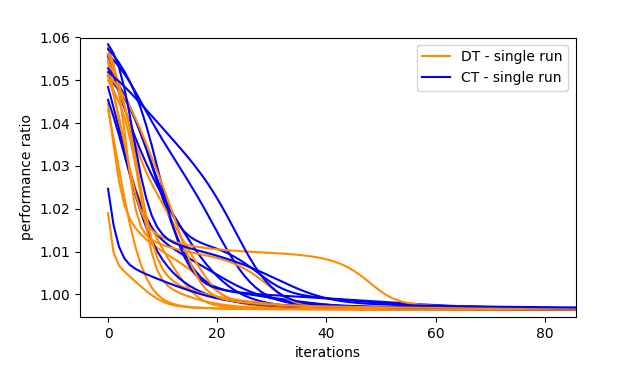
\includegraphics[width=1\linewidth]{img/ex1/g1.png}
  \captionof{figure}{Models convergences }
  \label{fig:sr50}
\end{minipage}
\begin{minipage}{1\textwidth}
  \centering
  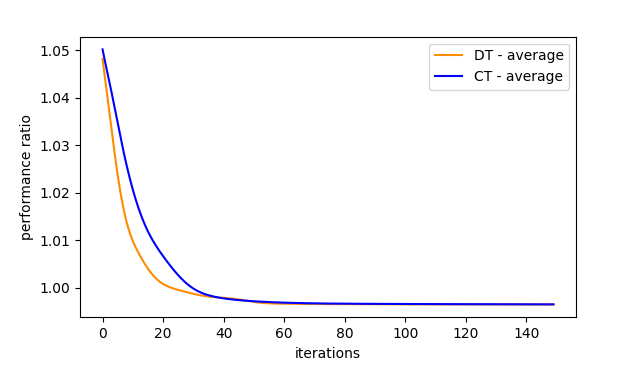
\includegraphics[width=1\linewidth]{img/ex1/g2.png}
  \captionof{figure}{Average of the convergences from various random starting points}
  \label{fig:avgc}
\end{minipage}
\end{figure} 

\begin{figure}
\centering
\begin{minipage}{1\textwidth}
  \centering
  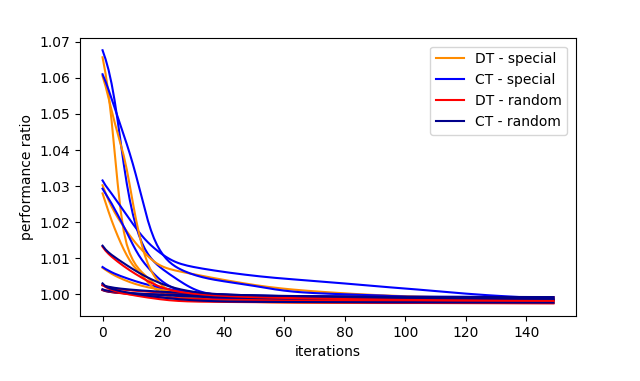
\includegraphics[width=1\linewidth]{img/ex1/g3.png}
  \captionof{figure}{Average of the convergences for various generated datasets}
  \label{fig:all}
\end{minipage}
\begin{minipage}{1\textwidth}
  \centering
  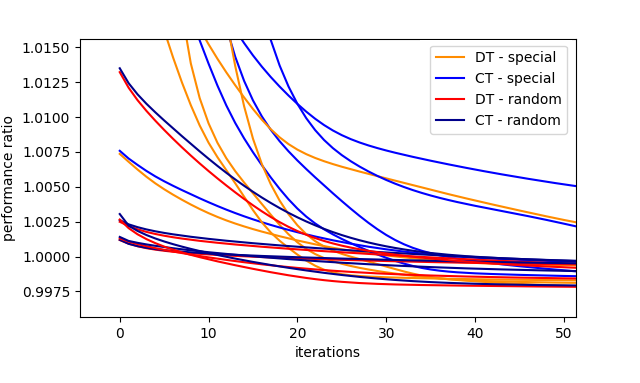
\includegraphics[width=1\linewidth]{img/ex1/g4.png}
  \captionof{figure}{Average of the convergences for various generated datasets (zoom)}
  \label{fig:random}
\end{minipage}
\end{figure}  

\subsection*{ Conclusions }

The slower convergence of continuous-time model is bounded with different character of the model. Since in the discrete-time model we always know the precise time when the state-change can happen (always at observation point), in continuous-time model it can happen in any time in between as well. Thus, computing of the new estimated parameters in maximization step needs to deal with more uncertainty. 
In continuous-time model is uncertainty not only caused by indirect observation of hidden states, but also by possible state changes in between of the observations. As we have any observations from that area, the probability estimation is counted by parameters from the last iteration, what is creating momentum in favor of old parameters and slow down the convergence process. The longer is the time interval, the stronger is the momentum.

In the second experiment we have showed, how characteristic of the searched model influenced training complexity. The randomly generated models usually generate datasets with higher entropy. Such datasets are closer to converge from most regions of the parameter space. 

The over-performing of the original model is caused by the overfitting. The small size of dataset was not sufficient to cover characteristic of the model completely, instead the trained models were learned to fit its imprecision. It is not a problem for our experiment as the original models were chosen more-less randomly and it fills in its purpose. The over-performing would probably gradually disappear with growing size of the data-set. It is shown in experiment \ref{sec:plast}.

All of the training conducted during this experiment converged close to global optima. We have used simple three-states models. Behavior of more complex models will be examined later in Section \ref{sec:high}.    


\section{Computational Complexity}\label{sec:cc}

In this section we are comparing time-performance of the float and integer-interval variants of CT-HMM  as described in implementation part \ref{sec:alg}.
In two following subsections we experiment with variable hidden states number and maximal time interval and examine, if the measured values correspond to their theoretical expectations described in Section \ref{sec:complex}.

\subsection{Variable Hidden States Number}

The hidden states number, referred to as $n$ is the key parameter in overall algorithm complexity. Due to computing of the matrix exponentials $\mathcal{O}(n^3)$ for every pair of end states, it influence the final time-complexity by its fifth power $n^5$. The upper bound theoretical complexity dependence on $n$ is the same for both of the variants. However, the float-algorithm counts the matrix exponential by \textit{expm} method separately for every time interval, while the integer-algorithm counts it only once and then use the matrix multiplication to get the individual results \ref{it:ctc}. In the experiment we measure and compare the times of most costly algorithm parts, and notice how big is the portion of the overall computational complexity consumed by them. 


\subsubsection*{ Description }

We have trained the models with the variable number of hidden states. To minimize the impact of the other factors, we have let the number of output variables to be constantly 10 and we have used the same randomly generated dataset for both algorithm variants. The integral times intervals were generated by exponential distribution with parameter 0.5. To minimize the time measurements error, we have always run 10 iterations of algorithm and repeated the overall procedure 5 times. 

To see how the size of the dataset influence time-demand, we have conducted all the described experiments twice. Once with the \textit{small} dataset - compounding 10 sequences of 10 observations and once with the \textit{big} dataset - compounding 10 sequences of 100 observations.  

\subsubsection*{ Observation }

In Figure \ref{fig:e2n}, we can observe that the float-interval algorithm is always slower. The prevalent source of complexity is the \textit{expm} method. In the float-interval algorithm over the small dataset are all other parts of the algorithm almost neglectable comparing to it.

Comparing to the \textit{expm} are the time-demands of \textit{square and multiply} algorithm considerably smaller. It is called multiple times over different time-intervals and still takes smaller portion of the time as the single \textit{expm} call.

The increase of the dataset size caused the larger gap among the whole algorithm time-complexity and its measured subparts - either \textit{expm} or the sum of \textit{expm} and \textit{square and multiply} depending on the algorithm \ref{fig:e2big}.   

\begin{figure}
\centering
\begin{subfigure}{1\textwidth}
  \centering
  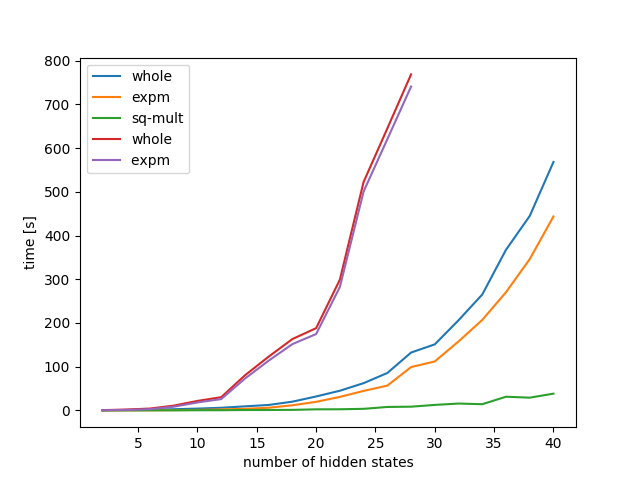
\includegraphics[width=1\linewidth]{img/ex2/small.png}
  \caption{Small dataset}
  \label{fig:e2small}
\end{subfigure}
\begin{subfigure}{1\textwidth}
  \centering
  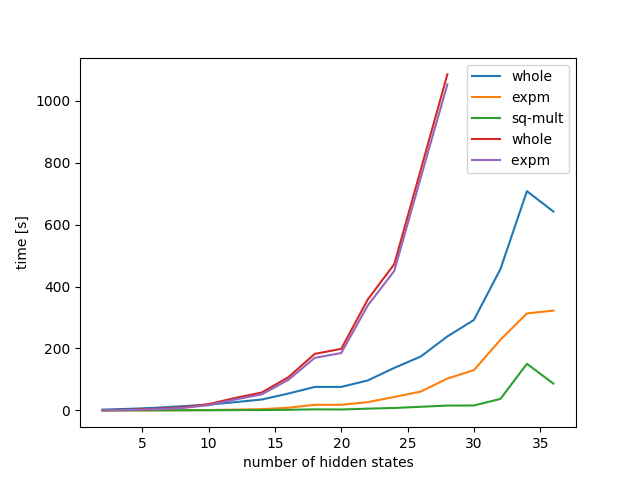
\includegraphics[width=\linewidth]{img/ex2/big.png}
  \caption{Big dataset}
  \label{fig:e2big}
\end{subfigure}
\caption{ Time-complexity of two algorithm variants and their subparts }
\label{fig:e2n}
\end{figure}

\subsubsection*{ Conclusion }

We have only changed the number of states and let the dataset to be the same, so the $t_{\max}$ parameter from the integer-interval complexity $\mathcal{O}(r n^5 \log(t_{\max}))$ is fixed as constant. This makes both algorithm variants to have same complexity $\mathcal{O}(r n^5)$. The measurements have shown, the big multiplicative constant of \textit{expm} method. That's way it is almost always better to use the integer-interval algorithm. (Its numerical stability is tested later in Section \ref{sec:ns}) 

The most of the computational power is used to count matrix exponentials $expm$. In most cases it is the predominant cause of algorithm "slowness". It makes not much sense to edge-optimize other parts of the algorithm. Instead, the faster implementation of \textit{expm}, its parallelization or replacement with other method could spare the significant portion of time.      

Training over the big dataset \label{fig:e2big} has decreased the percentage of the time spent by $expm$ method. It is because the higher demand of other algorithm parts. Potentially, it can happen that this gap would overgrowth the $expm$ part. The complexity of the algorithm part that call $expm$ method only depend on $r$ - the number of different time intervals, however there are parts of the algorithms with complexity ${O}(n^2T)$ \ref{it:ctc}, where $T$ is number of all time intervals. So for the huge dataset with lower number of hidden states and many identical time intervals can this part be the predominant cause of the complexity.   

\subsection{Variable Maximal Time Interval}

The other parameter presented in the theoretical time complexity of the integer-interval algorithm $\mathcal{O}(r n^5 \log(t_{\max}))$ is $t_{\max}$ - maximal length of the time interval. On the oder side the parameter is not part of the float-interval algorithm complexity term $\mathcal{O}(r n^5)$ \ref{it:ctc}. The experiment aims to observe how the variable value of $t_{\max}$ changes the computational demand of the algorithm.  


\subsubsection*{ Description }

In the experiment we have set $t_{\max}$ as the variable, taking values of powers of two from $2^1$ to $2^{56}$. The use of higher values (even floats) was impossible, because of conversion to 64-bites integer used in \textit{SciPy} \textit{expm} method, that eventually causes the integer overflow. We have generated the dataset of 10 sequences by 10 observations. There was always at least one time-interval of length $t_{\max}$ and all other were chosen uniformly from interval $[1,t_{\max}]$. We have trained the model of $10$ hidden states and $10$ observation variables. To smooth the influence of the time measurement imprecision, we have run $10$ iterations and repeated the whole experiment $5$ times.   

\subsubsection*{ Observation }

Contrary to initial expectation both float and integer interval algorithm computational times are growing seemingly logarithmically with increasing $t_{\max}$. The cause of growth in float-interval algorithm is \textit{expm} method, in integer-interval algorithm it is caused mainly by \textit{square and multiply} method. There is the steep growth of the float-interval algorithm time demand present for small $t_{\max}$ values.

\begin{figure}[h]


\centering
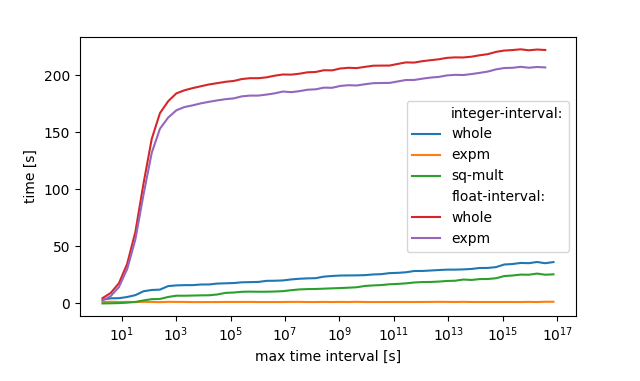
\includegraphics[width=1.0\linewidth]{img/ex2/log.png}
\captionof{figure}{Time-complexity of two algorithm variants and their subparts}
\label{fig:e2log}
\end{figure}

\subsubsection*{ Conclusion }

The steep growth at the beginning is caused by choice of integral interval lengths. For small values of $t_{\max}$ is higher probability of more same-sized time-intervals. That has direct impact at the complexity, where variable $r$ is directly present. The chance of choosing two same interval length for bigger $t_{\max}$ values is extremely low.

The logarithmic grow of \textit{square and multiply} method is obvious. But to explain similar behavior of the $expm$ method, we need to look deeper in its implementation \cite{al2009new}. 
The method is using Pad\'{e} approximants of different values from $3$ to $13$. The computation of the approximants of higher order is computationally more costly. The algorithm is choosing the smallest  Pad\'{e} approximant, which securely not overgrow the wished threshold error. Our observation suggest, that the bigger the numbers in the exponentiated matrix are, the bigger is the probability of the more complex Pad\'{e} approximant being chosen.

\section{Numerical Stability}\label{sec:ns} 

The main advantage of integer-interval variant of algorithm is that it computes costly matrix exponential only once and derive all other exponentials of the matrix multiplications by computing its powers, via \textit{square and multiply} method. It arise the question of numerical stability of the method. Can inaccuracies acquired by \textit{square and multiply} significantly change direction of convergence?   

\subsection*{ Description }
In the experiment we have run both integer and float-algorithms with same initial parameters. As the value of interest, we have measured the relative euclidean distance among both models jump-rates matrices $\matr{Q}$. We have used the models of $5$ hidden states and $5$ observable variables at the dataset of $100$ observation points. Time intervals were generated by exponential distribution with parameter $\lambda$ equal $0.1$, $0.01$ and $0.001$ consecutively. The obtained plotted error is the average value of $10$ runs of the experiment.      

\subsection*{ Observation }

The measured relative error of jump-rate matrices seems to grow faster at the beginning and gradually slowing its pace by growing iteration. Values of the relative error are very small. However it seems that the variance magnitude grows with the decreasing magnitude of exponential parameter $\lambda$. (Figures \ref{fig:l1},\ref{fig:l2},\ref{fig:l3})  


\begin{figure}
\centering
\begin{subfigure}{.9\textwidth}
  \centering
  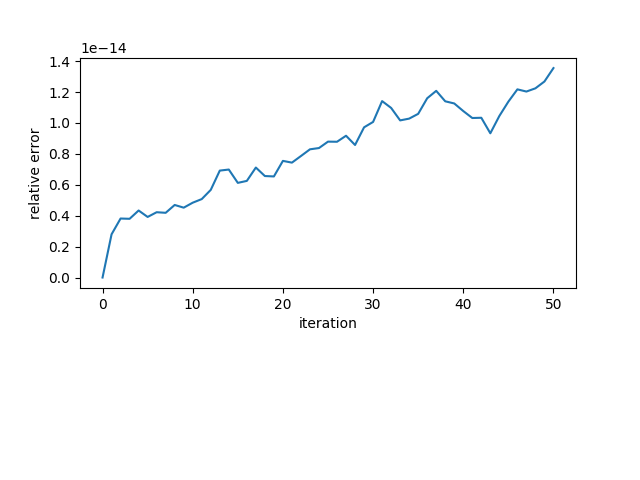
\includegraphics[width=1\linewidth]{img/ex3/0_1.png}
  \caption{ $\lambda = 0.1$ }
  \label{fig:l1}
\end{subfigure}
\begin{subfigure}{.9\textwidth}
  \centering
  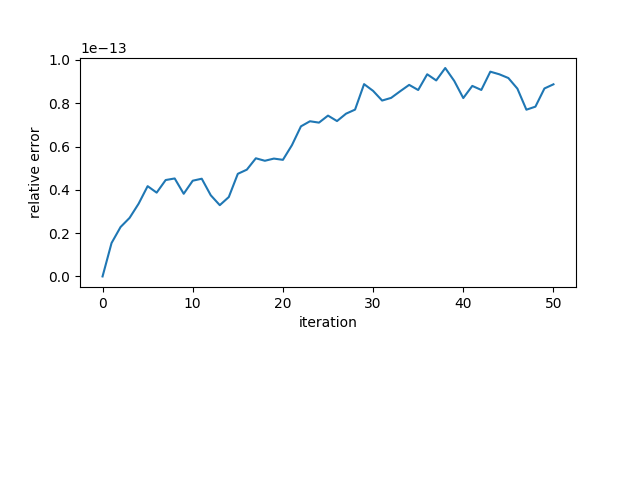
\includegraphics[width=1\linewidth]{img/ex3/00_1.png}
  \caption{$\lambda = 0.01$}
  \label{fig:l2}
\end{subfigure}
\begin{subfigure}{.9\textwidth}
  \centering
  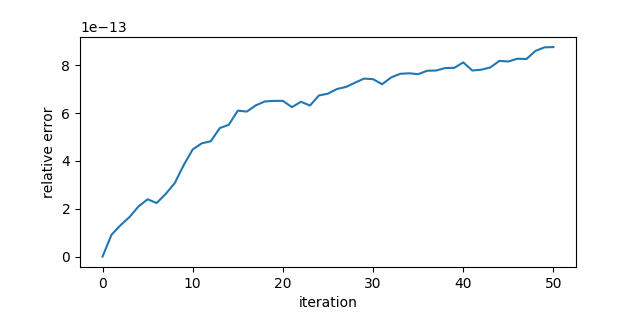
\includegraphics[width=1\linewidth]{img/ex3/000_1.png}
  \caption{$\lambda = 0.001$}
  \label{fig:l3}
\end{subfigure}
\caption{Relative distances of jump-rates matrices for data generated by exponential distribution with variable parameter $\lambda$}
\label{fig:test}
\end{figure}

\subsection*{ Conclusion }
The experiment haven't shown any significant error propagation. It has been a bit more prevalent at the beginning of the convergence as during this phase are the changes in the jump-rate matrices most prominent. Later errors seems to be eliminated as the solutions converging to the local optima. Probably, under some more extreme edge conditions the matrices may diverge. But, when taking into the account the randomness of the initial configuration and assorted characteristic of the parameter space, we do not see it as problem and we do not think it can, in general, negatively influence the performance of the algorithm. 

\section{Soft vs. Hard method}

This experiment compare the soft and the hard method of EM algorithm described in Section \ref{sec:shm}. The methods differ in their maximization function. The soft method maximize the probability of the dataset being generated by the model, whereas the hard method maximize the probability of the most likely state sequence generating the dataset. We have examined and compared the results of both these functions for both models.   

\subsubsection*{ Description }

There is any unified result of hard method trainings. Use of datasets generated by different models and also the various initial random parameters produce very different results. This makes the experimenting to be a complex task. In the observation we have tried to show the results uncovering most prevalent characteristics. First, we have measured the performance ratio on both training and testing dataset. We have chosen small tree hidden states model that was trained on the dataset of 100 sequences of 100 observation points as it manifests the methods characteristics sufficiently well.    

The goal of the second part was to explore the possible strong feature of the hard method - maximizing the probability of most likely state sequence. We have taken the most probable state sequence of the trained model and compared its probability of being generated by both trained and original model. Performance ratio is this probability divided by probability of most probable sequence generated by the original model.

\subsubsection*{ Observation }

On Figure \ref{fig:ds} we can see the resulting convergences of the first part of the experiment measured on the tasting dataset. Models trained by the soft method all converge relatively good. On the other side models trained by the hard method are unstable at the beginning and the final performance ratio depends heavily on the initial random generation of parameters.  

\begin{figure}
\centering

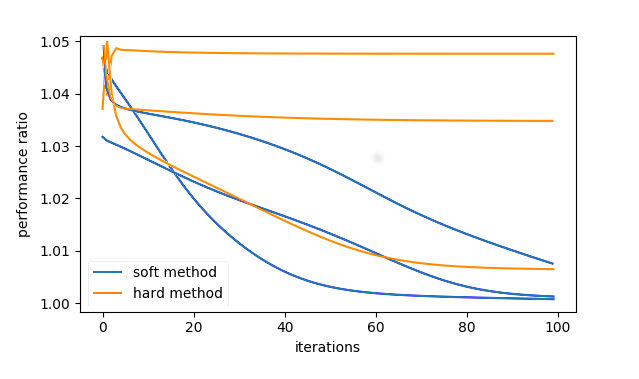
\includegraphics[width=1\linewidth]{img/ex4/b1.png}
\caption{Probability of the testing dataset being generating by the models}
\label{fig:ds}

\end{figure}

Figures \ref{fig:vit_all} show two different results of hard method convergence. While the probability of the most probable state sequence in both cases over-performed the original model, probability of the same sequence being generated by the original model is very low in the case on Figure \ref{fig:vit_bad}. The soft method behave more stable always producing intermediate results similar to the original model.

\begin{figure}
\centering
\begin{subfigure}{1.1\textwidth}
  \centering
  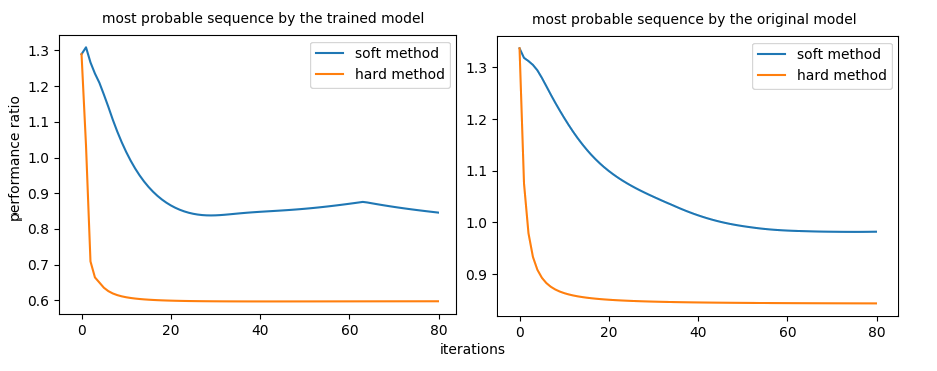
\includegraphics[width=1\linewidth]{img/ex4/hard_good.png}
  \caption{example of the hard method successful convergence}
  \label{fig:vit_good}
\end{subfigure}
\begin{subfigure}{1.1\textwidth}
  \centering
  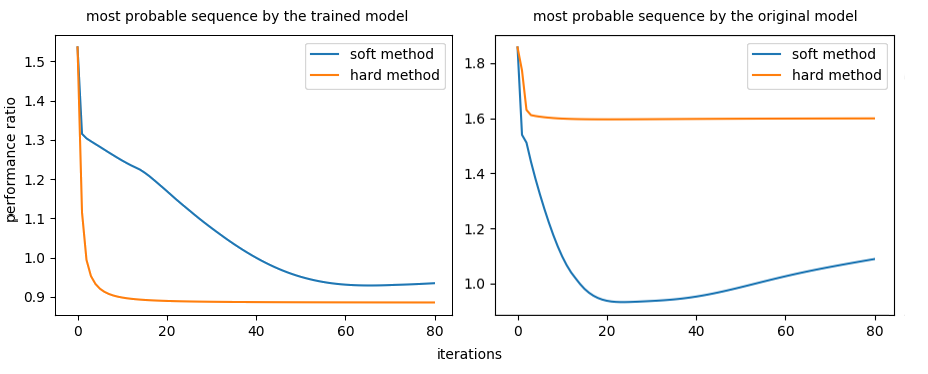
\includegraphics[width=1\linewidth]{img/ex4/hard_bad.png}
  \caption{example of the hard method misleading convergence}
  \label{fig:vit_bad}
\end{subfigure}
\caption{Performance ratio of the most probable state sequence }
\label{fig:vit_all}
\end{figure}

\subsubsection*{ Conclusion }
The hard method is maximizing the different likelihood function as described in Section \ref{sec:shm}. Its use for maximizing the probability of dataset being generated by the model is very unstable. Although sometimes it can produce satisfying results, it just appears as the side-effect of its original purpose.

The hard method behave considerably well in maximizing the probability of most probable state sequence. However, as the experiments uncovered, the resulting sequence has often very low probability of being generated by the original model, thus the models parameters are different.    

\section{Hidden States Number}\label{sec:hsn}

The number of hidden states is an important parameter, influencing the characteristic of the model. The higher number means the higher plasticity of the model. It can be beneficial as the model can better fit the domain space, however sometimes it may not be useful at all and cause the over-training. The parameter also critically influence the time and memory complexity of the algorithm. In following two experiments we observe, how variable number of states behave, when matching the dataset generating by single model, and in the later we try to find the limits of the algorithm regarding the number of states and examine how the increasing complexity of the parameter space influence the convergence ability.    

\subsection{Plasticity of the Models}\label{sec:plast}

\subsubsection*{ Description }
For this experiment we considered an artificial model consisting of five hidden states and four observation symbols arranged in the way of birth and death chain as in Figure \ref{fig:db}. There is not allowed for the model to change states except in the way of arrows. To add the uncertainty into the dataset, we have blurred the observation symbol emission by adding the $15\%$ error to the emitted symbol. The model is deliberately build in the way, so it uncovers the properties worthy to explore. However the properties are more or less visibly present in any model. 


\begin{figure}
\centering
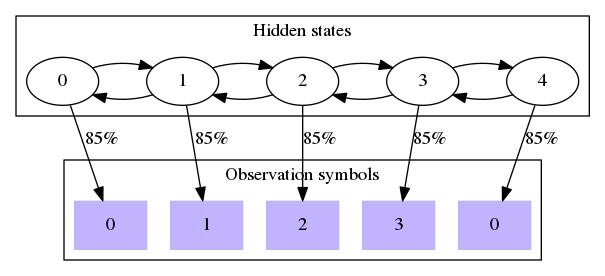
\includegraphics[width=1\linewidth]{img/ex5/hs.png}
\caption{Schema of the model ``birth and death'' }
\label{fig:db}
\end{figure}
 
We have generated three random datasets. The \textit{small} training dataset consisting of $15$ sequences each by $15$ observations and two \textit{big} datasets of $100$ sequences by $100$ observations, one for training and other for testing purpose. We have used both training datasets to train models with variable number of hidden states (from 2 to 8) and marked their performance after every of one hundred iteration at the respective training and \textit{big} testing dataset. We have repeated the experiments five times and plotted the average results.   

\subsubsection*{ Observation }

The models, except the ones with 2 and 3 hidden states, were able to over-perform the original model at the \textit{small} training dataset after couple of iterations \ref{fig:smtrain}. The bigger number of hidden states makes the convergence faster and also converge to the lower value. The measure at the testing dataset shows, that the models were actually over-fitted after couple of iterations and later diverge from the actual model. \ref{fig:smtest}. 

On the contrary the convergence lines plotting the training on the \textit{big} dataset \ref{fig:bgtrain} are almost the same as results on the testing data \ref{fig:bgtest}. Models with the hidden states number higher or equal 5 converge well. After one hundred iteration they have reached performances in interval $(1.00025,1.006)$ on the training dataset and $(1.0032,1.01)$ on the testing dataset. Higher number of states make the convergence faster, but all of the models seems to converge to the similar value. Models with the 4 or lower number of hidden states converge visibly worse. 

\begin{figure}
\centering
\begin{subfigure}{1\textwidth}
  \centering
  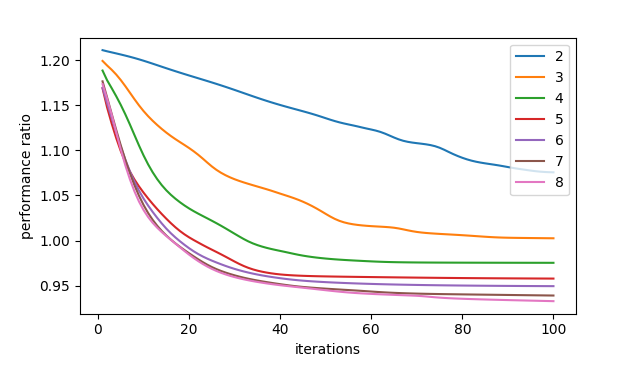
\includegraphics[width=1\linewidth]{img/ex5/small_train.png}
  \caption{Performance on the \textit{small} training dataset}
  \label{fig:smtrain}
\end{subfigure}
\begin{subfigure}{1\textwidth}
  \centering
  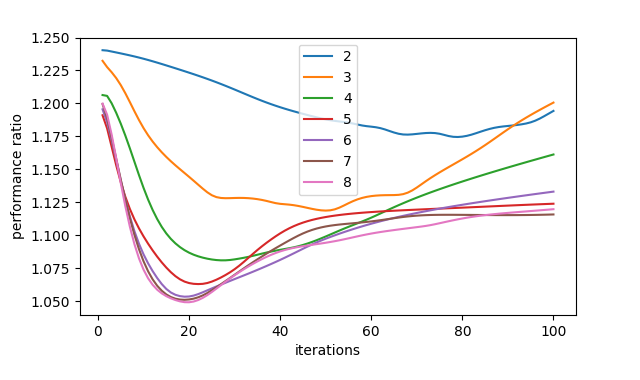
\includegraphics[width=1\linewidth]{img/ex5/small_test.png}
  \caption{Performance on the testing dataset}
  \label{fig:smtest}
\end{subfigure}
\caption{Performance of the models with variable hidden states number trained by the \textit{small} dataset}
\label{fig:sm}
\end{figure}

\begin{figure}
\centering
\begin{subfigure}{1\textwidth}
  \centering
  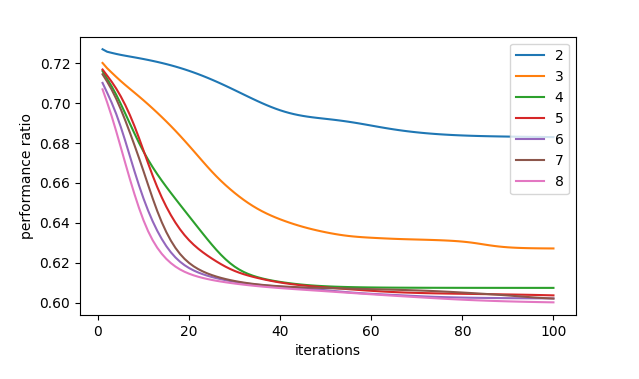
\includegraphics[width=1\linewidth]{img/ex5/big_train.png}
  \caption{Performance on the \textit{big} training dataset}
  \label{fig:bgtrain}
\end{subfigure}
\begin{subfigure}{1\textwidth}
  \centering
  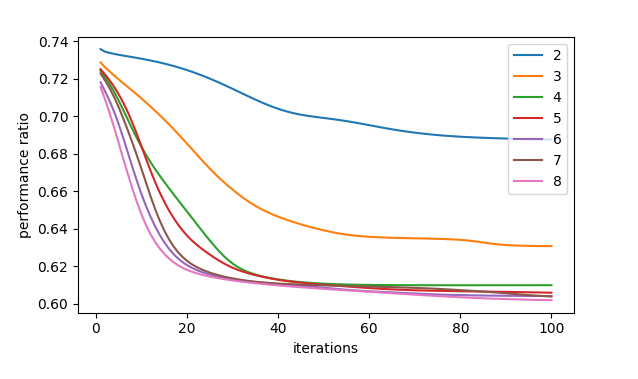
\includegraphics[width=1\linewidth]{img/ex5/big_test.png}
  \caption{Performance on the testing dataset}
  \label{fig:bgtest}
\end{subfigure}
\caption{Performance of the models with variable hidden states number trained by the \textit{big} dataset}
\label{fig:bg}
\end{figure}

\subsubsection*{ Conclusion }
Choosing the correct number of hidden states is crucial as its under-valuating can negatively influence the performance of the algorithm. Insufficient number of the hidden states for models 2-4 does not allow them to converge to the optimum values. The waves on the convergence lines of models 2 and 3 reveal that the averaged convergence lines differ. That marks the instability, thus the model that is too weak to cover the problem space. Model 4 was probably not able to distinguish the states at the ends of the birth and death sequence, that's way it has not reached the peak performance.

We haven't proof that the over-valuated number of hidden states makes the models more vulnerable to over-fitting, as all models has over-fitted similarly. The higher number of states than in the original model makes the model to converge in the smaller number of iterations, but not to the considerably better values. However, the cost of computationally more expensive single iteration makes their convergence slower in real time.

The experiment also stresses the importance of sufficiently sized dataset, as the small one emphasized the statistical error and lead to the over-fitting of the models. That is not the surprise, the weak dataset can't train powerful model. 

\subsection{High Number of Hidden States}\label{sec:high}

Training of models with high number of hidden states is computationally expensive. In this experiment we measure time demands of training for full and sparse jump-rate matrix as described in algorithm section \ref{sec:alg}. The second part of the experiment examines performance ratio and how it changes with the growing number of hidden states. 

\subsubsection*{ Description }

All datasets used in this experiment were generated by the model with ``birth and death'' sequence of hidden states (similar as in Figure \ref{fig:db}) always with the same number of hidden states and observation symbols as the trained models. The jump-rate matrix $\matr{Q}$ of such a model is three-diagonal. The actual jump rates in the nonzero positions were generated randomly.

As the training models we have used \textit{full} jump-rate matrix and \textit{sparse} (three-diagonal) jump-rate matrix. All parameters were initially randomly generated. In the first part of the experiment we have measured time of single iteration for models with full and sparse matrix.
For full matrix we have used models with 5 to 75 hidden states, for the sparse matrix models with 5 to 170 hidden states. We have used dataset of 1000 observation points.
 In the second part we have compared the convergence of models with full and sparse jump-rate matrix with variable number of hidden states. To overcome the overfitting we have used dataset of 10000 observation points.    

\subsubsection*{ Observation }

In Figure \ref{fig:time} we can see that also the models with the high number of hidden states are able to converge in feasible time. Sparsity of the jump-rate matrix is crucial for the algorithm speed. It is possible to make three iteration in a hour by model with full matrix of 75 hidden states and the same number of iterations by model with sparse matrix of 170 hidden states.   

The second part of the experiment in Figure \ref{fig:big} shows the results of the trained models on the testing dataset. The models with sparse jump-rate matrix converge significantly faster and reach the similar performance rate for all hidden states number. On the other hand the models with full jump-rate matrix are becoming a bit less plastic with growing number of hidden states.

\begin{figure}
\centering
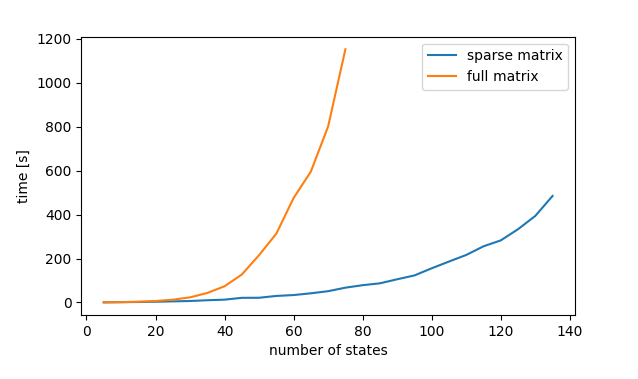
\includegraphics[width=1\linewidth]{img/ex5.2/time.png}
\caption{Time demands of single iteration }
\label{fig:time}
\end{figure}


\begin{figure}
\centering
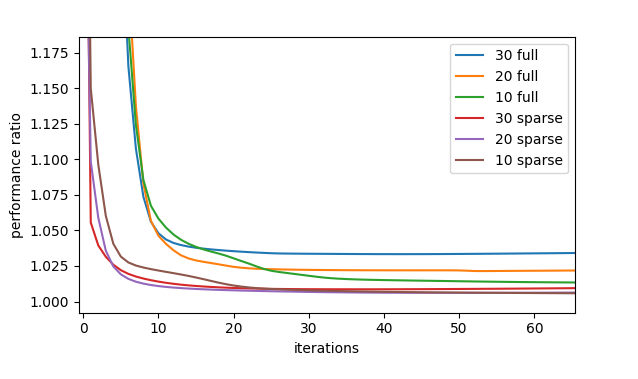
\includegraphics[width=1\linewidth]{img/ex5.3/big.png}
\caption{Convergences for full and sparse matrices with variable number of hidden states}
\label{fig:big}
\end{figure}

\subsubsection*{ Conclusion }

We have showed that the implemented algorithm is fast enough to train models with high number of hidden states. The use of the sparse jump-rate matrix can significantly shrink the time-demands and also produce faster and better convergence. We recommend to use the sparse matrix always, when the characteristic of the problem allows it and if we are sure that the transition between two states can't occur. 

The higher is the number of nonzero elements in the jump-rate matrix, the harder problem is need to be solved because convergence in multidimensional parameter space is more likely to fall in a local minima.  

\setsecnumdepth{part}
\chapter{Conclusion}

In this Master's thesis we provide detailed theoretical description of discrete-time and continuous-time hidden Markov models. We have examined general characteristic of CTHMM and explained how it differs from discrete-time model. Most emphases was given to continuous-time model learning methods, which various variants were described and implemented.   

We have created the first of its kind general purpose continuous-time hidden Markov model library under open-source license. The computationally effective and simple to use library provides broad functionality and implementation of current state-of-the-art algorithms for both discrete-time and continuous-time hidden Markov model. The most novel part are several variations of EM learning algorithm using method of matrix exponentiation for counting end-state conditioned expectations (\textit{expm}).

The implemented algorithms are able to handle hundreds of hidden states.  Fully connected model of 75 hidden states or sparse model of 170 hidden states can run one iteration of continuous-time learning algorithm in time under 20 minutes on 2.50GHz machine, when trained on the medium sized dataset.  

We have implemented two variants of the \textit{expm} algorithm different in the maximized likelihood function, so called soft and hard method. Soft method maximizes the probability of the training dataset being generated by the model, hard method uses the results of the Viterbi algorithm maximizing the most probable state sequence. We have showed the superiority of the soft method as the hard method is not directly optimizing the wished likelihood function and often produces misleading results.

The models trained on the dataset with integer lengths of time intervals can benefit from \textit{intege-interval} variant of algorithm sparing the number of matrix exponential computations, which as we have showed is the most time demanding part of the algorithm. The experiments referring to its numerical stability demonstrated that the relative error is negligible to negatively influence the computation, whereas the time demands decreased radically.  

\section{Future Work}

The effective algorithm for the continuous-time hidden Markov model parameters learning is relatively new. It has showed to be successful in biomedical field, but it certainly could be applied to solve different domains. The open-source library may help to spread the method to the broader range of data scientist with different fields of interests. 

The functionality of the library can be further increased. Either by looking for the new convergence methods or implementing the model extension (for example continuous or multiple observations).

It would be interesting to examine CT-HMM comparing to recurrent neural network as they share some common characteristics. Possibly some hybrid method could be developed. 

\bibliographystyle{iso690}
\bibliography{bibliography}

\setsecnumdepth{all}
\appendix

\chapter{Acronyms}
% \printglossaries
\begin{description}
	\item[CL] Complete Likelihood
	\item[CT-HMM] Continuous-time Hidden Markov Model
	\item[CTMP] Continuous-time Markov Process
	\item[DP] Dynamic Programming
	\item[DT-HMM] Discrete-time Hidden Markov Model	
	\item[DTMP] Discrete-time Markov Process	
	\item[EM] Expectation-Maximization
	\item[HMM] Hidden Markov Model 
	\item[MLE] Maximum Likelihood Estimation
	
\end{description}


\chapter{Contents of enclosed CD}

%change appropriately

\begin{figure}

\dirtree{%
.1  .
.2 readme.txt\DTcomment{brief description of the CD content}.
.2 HMMs\DTcomment{hidden Markov models library}.
.3 hmms\DTcomment{source files}.
.4 cthmm.pyx\DTcomment{continuous-time hidden Markov model class}.
.4 dthmm.pyx\DTcomment{discrete-time hidden Markov model class}.
.4 art.py\DTcomment{additional functions for visualization}.
.4 train.py\DTcomment{additional functions for multi-training}.
.3 docs\DTcomment{documentation files}.
.3 tests\DTcomment{testing and experiment files}.
.4 experiments.py \DTcomment{source code for experiments}.
.3 hmms.ipynb \DTcomment{interactive tutorial}.
.3 setup.py \DTcomment{installation script}.
.3 README.md \DTcomment{description of the library}.
.2 text\DTcomment{text of the thesis}.
.3 DP\_Lopatovsky\_Lukas\_2017.tex\DTcomment{text of the thesis in latex}.
.3 DP\_Lopatovsky\_Lukas\_2017.pdf\DTcomment{text of the thesis in pdf}.
.3 img\DTcomment{images and data files to experiments}.
}
	
\end{figure}

\end{document}
